\chapter{Dynamic Model of Underwater Robots}
\label{Appendix:DM}
An accurate model of the underwater robot dynamics plays a decisive role for designing controller for underwater robots. Especially for the computational design of the underwater robots, the vehicle dynamics is varying in each optimization loop, because the geometric variables are always updated and consequently the parameters in the robot dynamics are changed. Therefore, it is necessary to identify all robot dynamic parameters and derive them systematically. In this chapter, we firstly focus on the kinematics of underwater robots, i.e., on the translational and rotational motions of underwater robots without consideration of causes of motions. Then hydrodynamic effects (added mass and hydrodynamic damping) and the restoring forces (gravity and buoyancy) are taken into consideration to derive the dynamic model for underwater robots.  

For all the variables relating to underwater robots (position, velocity, acceleration, forces, moments), we use the following standard representation as depicted in Table \ref{table:SN}.
\begin{table}[h]
\centering
\caption{Standard notation of underwater robot}
\begin{tabular}{| l | l | l | p{2cm} |}
\hline
\textit{\textbf{translational motion}}&\textit{\textbf{position}}&\textit{\textbf{linear velocity}}&\textit{\textbf{force}} \\ \hline
surge~(motion in x-direction)&$  x$&$  u$&$ X $ \\ \hline
sway~(motion in y-direction)&$  y$&$ v $&$ Y $ \\ \hline
heave~(motion in z-direction)&$  z$&$  w$&$  Z$ \\ \hline
\textit{\textbf{rotational motion}}&\textit{\textbf{Euler angle}}&\textit{\textbf{angular velocity}}&\textit{\textbf{moment}} \\ \hline
roll~(rotation about x-axis)&$ \phi $&$  p$&$ K $ \\ \hline
pitch~(rotation about y-axis)&$ \theta $&$  q$&$ M $ \\ \hline
yaw~(rotation about z-axis)&$ \psi $&$  r$&$ N $ \\ \hline
\end{tabular}
\label{table:SN}
\end{table}   
\section{Kinematics of Underwater Robots}
\subsection{Reference Frames and Basic Notations}
A world inertial frame $\left\{ i \right\}=(x_{i},y_{i},z_{i})$ describes the environment of the underwater robot which is fixed in space. Stationary objects like the walls of basin, which enter the fluid mechanics as boundary conditions, are fixed in space and therefore independent of time. The world coordinate frame is defined in such a way that the directions $x_{i}$ and  
$y_{i}$ are in the plane of the undisturbed water surface and $z_{i}$ is in the positive direction pointing downwards into the fluid~\cite{Vollmayr2014}.

The body-fixed reference frame $\left\{ b \right\}=(x_{b},y_{b},z_{b})$ is a moving coordinate frame fixed to the robot. The origin $o_{b}$ is usually chosen to coincide with the geometric center of hull which will be referred to as CO. The longitudinal axis $x_{b}$ is directed from aft to fore, the transversal axis $y_{b}$ is directed to starboard and the normal axis $z_{b}$ orientates from top to bottom. 
\begin{figure}
\includegraphics[width=\textwidth]{Frames.eps}
\caption{Inertial world frame $\left\{ i \right\}$ and body frame $\left\{ b \right\}$}	
\label{FIG:FM}
\end{figure}

The rotation matrix transforming quantities (linear velocities, forces and moments) in inertial frame $\left\{ b \right\}$ to body frame $\left\{ i \right\}$ are denoted as $\emph{\textbf{R}}$, and they are elements in $\textit{SO(3)}$ belonging to \textit{special orthogonal group of order 3:}
\begin{align}
\textit{SO(3)}=\left\{ \emph{\textbf{R}}|\emph{\textbf{R}}\in\mathbf{R}^{3\times3}, \emph{\textbf{R}}\emph{\textbf{R}}^{T}=\emph{\textbf{R}}^{T}\emph{\textbf{R}}=\emph{\textbf{I}}, det(\emph{\textbf{R}})=1\right\}.
\end{align}

The vector cross-product $\times$ is defined by
\begin{align}
\vec{\zeta} \times \vec{a}:=\emph{\textbf{S}}(\vec{\zeta})\vec{a},
\end{align}
where $\emph{\textbf{S}}$ is a skew-symmetrical matrix satisfying $\emph{\textbf{S}}=\emph{\textbf{S}}^{T}$ and defined as
\begin{align}
\emph{\textbf{S}}(\vec{\zeta})=-\emph{\textbf{S}}^{T}(\vec{\zeta})=\begin{pmatrix}
0&-\zeta_{3}&\zeta_{2}\\
\zeta_{3}&0&-\zeta_{1}\\
-\zeta_{2}&\zeta_{1}&0
\end{pmatrix}, \vec{\zeta}=\begin{pmatrix}
\zeta_{1}\\
\zeta_{2}\\
\zeta_{3}
\end{pmatrix}.\label{EQ:CrossProduct}
\end{align}

The rotation matrix $\emph{\textbf{R}}_{\zeta,\bigskip \beta}$ corresponds to a rotation of angle $\beta$ in the counter-clockwise direction about a rotation axis parallel to the unit vector $\vec{\zeta}=[\zeta_{1}, \zeta_{2}, \zeta_{3}]^{T}, ||\zeta||=1$:
\begin{align}
 \emph{\textbf{R}}_{\zeta,\bigskip \beta}=\emph{\textbf{I}}_{3\times 3}+\sin(\beta)\emph{\textbf{S}}(\vec{\zeta})+[1-\cos(\beta)]\emph{\textbf{S}}^{2}(\vec{\zeta}), \label{EQ:BS3}
 \end{align} 
where $\emph{\textbf{I}}_{3\times 3}$ is the three-dimensional identity matrix. Because $\vec{\zeta}$ is a unit vector, $\emph{\textbf{S}}^{2}(\vec{\zeta})=\vec{\zeta}\vec{\zeta}^{T}-\emph{\textbf{I}}_{3\times 3}$.

While the position and orientation of underwater robots are expressed with respect to inertial frame $\left\{ i \right\}$, the linear and angular velocities of underwater robots are conventionally expressed relative to body frame $\left\{ b \right\}$.  
The position of underwater robots in the inertial world frame $\left\{ i \right\}$ is denoted by the vector 
\begin{align}
\vec{p}=
\begin{pmatrix}
x\\y\\z
\end{pmatrix}
\in 
\mathbb{R}^{3},
\end{align}
the orientation of underwater robots is described by Euler angles
\begin{align}
\vec{\lambda}=
\begin{pmatrix}
\phi \\ \theta\\ \psi
\end{pmatrix}
\in 
\mathit{S}^{3},
\end{align}
where $\mathbb{R}^{3}$ is the three dimensional Euclidean space and $\mathit{S}^{3}$ is a sphere. We can write them together into a six-dimensional generalized position vector $\vec{\eta}\in \mathbf{R}^{3}\times\mathit{S}^{3}$:
\begin{align}
\vec{\eta}=
\begin{pmatrix}
\vec{\eta}_{1}\\
\vec{\eta}_{2}
\end{pmatrix}=
\begin{pmatrix}
\vec{p} \\
\vec{\lambda}
\end{pmatrix}.
\end{align}
 
The body-fixed linear velocity which is the linear velocity of $o_{b}$ relative to world frame $\left\{ i \right\}$ expressed in body frame $\left\{ b \right\}$ is denoted by the vector 
\begin{align}
\vec{v}^{b}_{b/i}=
\begin{pmatrix}
u\\v\\w
\end{pmatrix}
\in
\mathbb{R}^{3}.
\end{align}
In other words, $\vec{v}^{b}_{b/i}$ denotes the changing of length of vector $o_{i}o_{b}$ observed in body frame $\left\{ b \right\}$, where $o_{i}$ and $o_{b}$ are the origin of inertial world frame $\left\{ i \right\}$ and body frame $\left\{ b \right\}$, respectively.   

The body-fixed angular velocity which is the angular velocity with respect to world axes $\left\{ i \right\}$ expressed in $\left\{ b \right\}$ is denoted by the vector
\begin{align}
\vec{\omega}^{b}_{b/i}=
\begin{pmatrix}
p\\q\\r
\end{pmatrix}
\in
\mathbb{R}^{3}.
\end{align}

Define a new generalized velocity vector $\vec{\upsilon}\in \mathbb{R}^{6}$: 
\begin{align}
\vec{\upsilon}=
\begin{pmatrix}
\vec{\upsilon}_{1}\\
\vec{\upsilon}_{2}
\end{pmatrix}
=\begin{pmatrix}
\vec{v}^{b}_{b/i} \\
\vec{\omega}^{b}_{b/i}
\end{pmatrix}.
\end{align}

The body-fixed forces and moments through $o_{b}$
are expressed by 
\begin{align}
\vec{f}^{b}_{b}=
\begin{pmatrix}
X\\Y\\Z
\end{pmatrix}
\in
\mathbb{R}^{3}
\end{align}
and
\begin{align}
\vec{m}^{b}_{b}=
\begin{pmatrix}
K\\M\\N
\end{pmatrix}
\in
\mathbb{R}^{3},
\end{align}
respectively.

The generalized force vector $\vec{\tau}\in \mathbb{R}^{6}$ is defined as
\begin{align}
\vec{\tau}=
\begin{pmatrix}
\vec{f}^{b}_{b} \\
\vec{m}^{b}_{b}
\end{pmatrix}.
\end{align}

Principal Rotations are rotations about $x$, $y$ and $z$ axes by setting $\vec{\lambda}=[1, 0, 0]^{T}$, $\vec{\lambda}=[0, 1, 0]^{T}$, and $\vec{\lambda}=[0, 0, 1]^{T}$ and $\beta=\phi$, $\beta=\theta$ and $\beta=\psi$, receptively. For simplicity, we use the following abbreviated notions for triangular functions:
\begin{align}
\sin(\cdot)=s(\cdot),
\end{align}
\begin{align}
\cos(\cdot)=c(\cdot),
\end{align}
\begin{align}
\tan(\cdot)=t(\cdot).
\end{align}
Using formula \ref{EQ:BS3}, we can get
\begin{align}
\emph{\textbf{R}}_{x,\phi}=\begin{pmatrix}
1&0&0\\
0&c \phi&-s \phi\\
0&s \phi&c \phi
\end{pmatrix},
\end{align}
\begin{align}
\emph{\textbf{R}}_{y,\theta}=\begin{pmatrix}
c \theta&0&s \theta\\
0&1&0\\
-s \theta&0&c \theta
\end{pmatrix},
\end{align}
\begin{align}
\emph{\textbf{R}}_{z,\psi}=\begin{pmatrix}
c \psi&-s \psi&0\\
s \psi&c \psi&0\\
0&0&1
\end{pmatrix}.
\end{align}
The Euler angles, roll($\phi$), pitch($\theta$) and yaw($\psi$), is written as vector $\vec{\lambda}=(\phi, \theta, \psi)^{T}$. For transformation from world frame $\lbrace i \rbrace$ to body frame $\lbrace b \rbrace$ it is customary to use the $zyx$ convention based on the Euler angles $\phi$, $\theta$ and $\psi$. 
\begin{align}
\emph{\textbf{R}}^{-1}(\vec{\lambda})&:=\emph{\textbf{R}}_{z, \psi}\emph{\textbf{R}}_{y, \theta}\emph{\textbf{R}}_{x, \phi} \nonumber \\
&=\begin{pmatrix}
c\psi c\theta&-s\psi c\phi+c\psi s\theta s\phi&s\psi s\phi+c\psi c\phi s\theta \\
s\psi c\theta&c\psi c\phi+s\phi s\theta s\psi&-c\psi c\phi+s\theta s\psi c\phi\\
-s\theta&c \theta s \phi&c \theta c\phi
\end{pmatrix}
\end{align}
and the inverse transformation from body frame $\left\{ b \right\}$ to world frame $\left\{ i \right\}$ is characterized by the rotation matrix:
\begin{align}
\emph{\textbf{R}}(\vec{\lambda})=\emph{\textbf{R}}^{-T}(\vec{\lambda})=\emph{\textbf{R}}_{x, \phi}^{T}\emph{\textbf{R}}_{y, \theta}^{T}\emph{\textbf{R}}_{z, \psi}^{T}
\end{align}
\begin{figure}
\centering
\includegraphics[width=0.6\textwidth]{Rotation1.eps}
\caption{Rotation over yaw angle $\psi$ about $z_{3}$. Note that $w_{3}=w_{2}$}	
\label{FIG:Rotation1}
\end{figure}
\begin{figure}
\centering
\includegraphics[width=0.9\textwidth]{Rotation2.eps}
\caption{Rotation over pitch angle $\theta$ about $y_{2}$. Note that $v_{3}=v_{2}$}	
\label{FIG:Rotation2}
\end{figure}
\begin{figure}
\centering
\includegraphics[width=0.7\textwidth]{Rotation3.eps}
\caption{Rotation over roll angle $\phi$ about $x_{1}$. Note that $u_{1}=u$}	
\label{FIG:Rotation3}
\end{figure}

The derivative of underwater robot position can be related to the body-fixed velocity vector $\vec{v}^{b}_{b/i}$
\begin{align}
\dot{\vec{p}}=\emph{\textbf{R}}(\vec{\lambda})\vec{v}^{b}_{b/i}.
\end{align}

The inverse transformation is 
\begin{align}
\vec{v}^{b}_{b/i}=\emph{\textbf{R}}^{-1}(\vec{\lambda})\dot{\vec{p}}.
\end{align}

In terms of relationship between body-fixed angular velocity $\vec{\omega}_{b/i}^{b}$ and the Euler rate $\dot{\vec{\lambda}}=(\dot{\phi}, \dot{\theta}, \dot{\psi})^{T}$ another transformation matrix $\emph{\textbf{Q}}(\vec{\lambda})$ is used. 
By expanding the following relationship
\begin{align}
\vec{\omega}_{b/i}^{b}=
\begin{pmatrix}
\dot{\phi}\\0\\0
\end{pmatrix}+
\emph{\textbf{R}}^{T}_{x,\phi}
\begin{pmatrix}
0\\ \dot{\theta}\\0
\end{pmatrix}+
\emph{\textbf{R}}^{T}_{x,\phi}\emph{\textbf{R}}^{T}_{y,\theta}
\begin{pmatrix}
0\\0\\ \dot{\psi}
\end{pmatrix}
:=\emph{\textbf{Q}}^{-1}(\vec{\lambda})\dot{\vec{\lambda}}
\end{align}
we can yield
\begin{align}
=\emph{\textbf{Q}}^{-1}(\vec{\lambda})
\begin{pmatrix}
1&0&-s\theta \\
0&c \phi&c \theta s \phi \\
0&-s \phi&c \theta c\phi
\end{pmatrix},\label{EQ:ATS1}
\end{align}
and
\begin{align}
\emph{\textbf{Q}}(\vec{\lambda})=
\begin{pmatrix}
1&s \phi t \theta&c \phi t\theta \\
0&c \phi&-s \phi \\
0&s \phi/c \theta&c \phi/ c\theta
\end{pmatrix}\label{EQ:ATS2}
\end{align}
Notice that $\emph{\textbf{Q}}(\vec{\lambda})$ is undefined for pitch angle of $\theta \neq \pm 90^{\circ}$. With help of \ref{EQ:ATS2} we can obtain
\begin{align}
\dot{\vec{\lambda}}=\emph{\textbf{Q}}(\vec{\lambda})\vec{\omega}^{b}_{b/i}.
\end{align}

The inertial world frame $\left\{ i \right\}$ is a frame of reference with homogeneous and isotropic description of time and space in a time-dependent manner. Newton's second law and Euler's law are formulated in inertial frame $\left\{ i \right\}$.

Note that vectors are always coordinate-free which means vectors exist without any defined frame and their length and direction stay invariant for all frames. When a vector is observed in a arbitrary frame, it should be decoupled as a linear combination of unit basis vectors of this frame. Thus, a vector is represented differently in terms of coordinates in different frames. 

The unit vectors  $\vec{i}_{b}$, $\vec{j}_{b}$ and $\vec{k}_{b}$ denote unit basis vectors of body-fixed frame $\left\{ b \right\}$. The unit vectors  $\vec{i}_{i}$, $\vec{j}_{i}$ and $\vec{k}_{i}$ denote unit basis vectors of the inertial world frame $\left\{ i \right\}$. For rotation of a body frame relative to an inertial frame, we can derive the relationship of coordinates of an arbitrary vector in $\left\{ i \right\}$ and $\left\{ b \right\}$.

Firstly, we study this problem in a simplified two-dimensional case. Assume the body-fixed frame $\left\{ b \right\}$ rotates about the z axis of the inertial frame $\left\{ i \right\}$ with a constant angular velocity $\omega_{z,\theta}$, $\theta=\omega_{z,\theta}t$ and these two frames coincide at time $t=0$. Conversion between coordinates $(x_{i}, y_{i})$ and $(x_{b}, y_{b})$ can be performed as follows:
 \begin{align}
x_{i}=x_{b}\cos\theta-y_{b}\sin\theta,
\end{align}
\begin{align}
y_{i}=x_{b}\sin\theta+y_{b}\cos\theta,
\end{align}
\begin{align}
x_{b}=x_{i}\cos(-\theta)-y_{i}\sin(-\theta),
\end{align}
\begin{align}
y_{b}=x_{i}\sin(-\theta)+y_{i}\cos(-\theta).
\end{align}
The unit vectors $\vec{i}_{b}$ and $\vec{j}_{b}$ can be represented by coordinates in body frame $\left\{ b \right\}$:
\begin{align}
\vec{i}_{b}^{b}=(1,0),
\end{align}
\begin{align}
\vec{j}_{b}^{b}=(0,1).
\end{align}
If we represent them with coordinates in inertial frame $\left\{ i \right\}$, we can obtain
\begin{align}
\vec{i}_{b}^{i}=(\cos\theta,\sin\theta),
\end{align}
and
\begin{align}
\vec{j}_{b}^{i}=(-\sin\theta,\cos\theta).
\end{align}

Take derivative of $\vec{i}_{b}$ and $\vec{j}_{b}$ in the inertial frame $\left\{ i \right\}$:
\begin{align}
\frac{^{i}d}{dt}\vec{i}_{b}=\frac{d}{dt}(\cos\theta\vec{i}_{i}+\sin\theta\vec{j}_{i})
=\frac{d\theta}{dt}(-\sin\theta\vec{i}_{i}+\cos\theta\vec{j}_{i})
=\omega_{z,\theta}\left(-\sin\theta,\cos\theta\right)=\omega_{z,\theta}\vec{j}_{b},
\end{align}
\begin{align}
\frac{^{i}d}{dt}\vec{j}_{b}=\frac{d}{dt}(\cos\theta\vec{i}_{i}+\sin\theta\vec{j}_{i})
=\frac{d\theta}{dt}(-\sin\theta\vec{i}_{i}+\cos\theta\vec{j}_{i})
=\omega_{z,\theta}\left(-\sin\theta,\cos\theta\right)=-\omega_{z,\theta}\vec{i}_{b}.
\end{align}
Define the rotation vector $\vec{\omega}_{b/i}=(0, 0, \omega_{z,\theta})$,
\begin{align}
 \dfrac{^{i}d}{dt}\vec{u}=\vec{\omega}_{b/i}\times \vec{u},
 \end{align} 
where $\vec{u}$ is either $\vec{i}_{b}$ or $\vec{j}_{b}$. This relationship can be extended to the three-dimensional rotation in space, that is, $\vec{u}$ can be $\vec{i}_{b}$, $\vec{j}_{b}$ or $\vec{k}_{b}$ and $\vec{\omega}_{b/i}$ is the angular velocity vector for rotation from $\left\{ i \right\}$ to $\left\{ b \right\}$ in space.

Assume an arbitrary vector $\vec{a}$, if we observe it in body frame $\left\{ b \right\}$, we can write it as linear combination of unit vectors of $\left\{ b \right\}$,
\begin{align}
\vec{a}(t)=a_{x}(t)\vec{i}_{b}+a_{y}(t)\vec{j}_{b}+a_{z}(t)\vec{k}_{b}.
\end{align} 
Differentiate of $\vec{a}$ with respect to time in the world frame $\left\{ i \right\}$:
\begin{align}
\dfrac{^{i}d}{dt}\vec{a}&=\dfrac{d a_{x}}{dt}\vec{i}_{b}+\dfrac{^{i}d\vec{i}_{b}}{dt}a_{x}+\dfrac{d a_{y}}{dt}\vec{j}_{b}+\dfrac{^{i}d\vec{j}_{b}}{dt}a_{y}+\dfrac{d a_{z}}{dt}\vec{k}_{b}+\dfrac{^{i}d\vec{k}_{b}}{dt}a_{z} \nonumber \\
&=\dfrac{d a_{x}}{dt}\vec{i}_{b}+\dfrac{d a_{y}}{dt}\vec{j}_{b}+\dfrac{d a_{z}}{dt}\vec{k}_{b}+[\vec{\omega}_{ib}\times
(a_{x}\vec{i}_{b}+a_{y}\vec{j}_{b}+a_{z}\vec{k}_{b})] \nonumber \\
&=\frac{^{b}d}{dt}\vec{a}+\vec{\omega}_{b/i}\times \vec{a}.
\end{align}
The following formula can be obtained:
\begin{align}
\frac{^{i}d}{dt}\vec{a}=\frac{^{b}d}{dt}\vec{a}+\vec{\omega}_{b/i}\times \vec{a}\label{EQ:VectorDerivative},
\end{align}
and this formula will be repeatedly used in following sections for derivation of the underwater robot dynamics.

Assume point A is an arbitrary point in the rigid robot body.
\begin{figure}
\centering
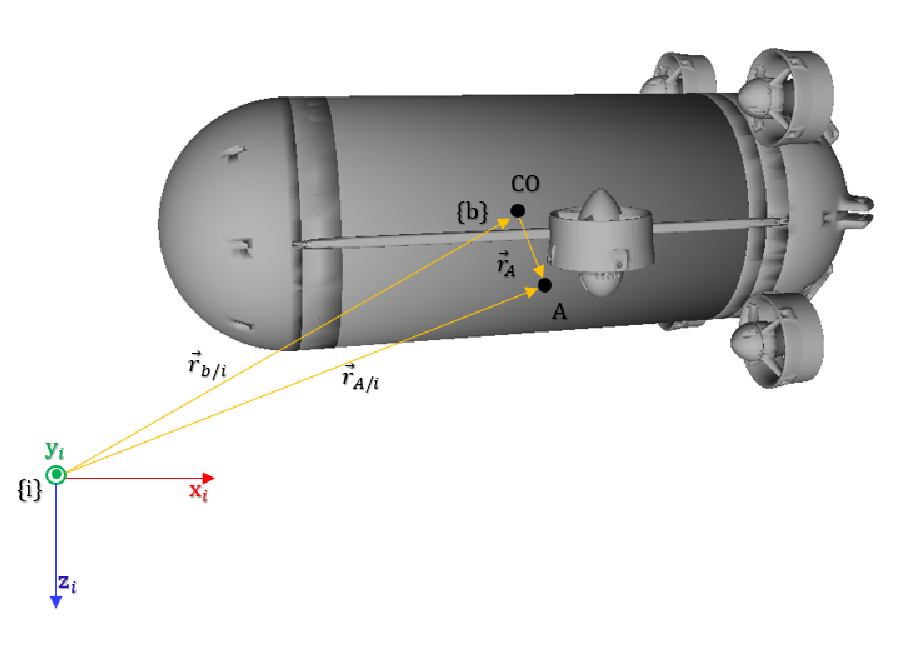
\includegraphics[width=\textwidth]{VectorRelation.eps}
\caption{Definition of vectors $\vec{r}_{A/i}$, $\vec{r}_{b/i}$ and $\vec{r}_{A}$}	
\label{FIG:VectorRelation}
\end{figure}
From Figure \ref{FIG:VectorRelation} we obtain 
\begin{equation}
\vec{r}_{A/i}=\vec{r}_{b/i}+\vec{r}_{A},
\end{equation}
where $\vec{r}_{A}$ is the distance from CO to A which denotes the location of the point A in body frame $\left\{ b \right\}$. 
Time differentiation of $\vec{r}_{A/i}$ in the inertial world frame $\left\{ i \right\}$ using \ref{EQ:VectorDerivative} gives
\begin{align}
\vec{v}_{A/i}=\dfrac{^{i}d}{dt}(\vec{r}_{A/i})
&=\dfrac{^{i}d}{dt}(\vec{r}_{b/i}+\vec{r}_{A}) \nonumber \\
&=\dfrac{^{i}d}{dt}\vec{r}_{b/i}+\dfrac{^{i}d}{dt}\vec{r}_{A} \nonumber \\
&=\vec{v}_{b/i}+ (\frac{^{b}d}{dt}\vec{r}_{A}+\vec{\omega}_{b/i}\times \vec{r}_{A}). \label{EQ:TM1}
\end{align}
A fixed point A in the rigid robot body satisfies 
\begin{align}
\frac{^{b}d}{dt}\vec{r}_{A}=\vec{0}.
\end{align}
Thus, the equation \ref{EQ:TM1} can be written as
\begin{align}
 \vec{v}_{A/i}= \vec{v}_{b/i}+ \vec{\omega}_{b/i}\times \vec{r}_{A}\label{EQ:VelocityTransformation}.
\end{align} 
This relationship is of great significance for further work, since it can be used to calculate the velocity at an arbitrary point A in the robot body from the translational velocities vector $\vec{v}_{b/i}$, the angular velocities vector $\vec{\omega}_{b/i}$ and the position vector $r_{A}$ denoting the position of point A in body frame $\left\{ b \right\}$. 
\subsection{Newton-Euler Equations of Motion about CG}
Newton's second law describes the relationship between the force exerted on the body $\vec{f}_{g}$ with the generated linear acceleration $\dot{\vec{v}}_{g/i}$. The resultant force acts on the center of gravity CG. Having implemented Newton's second law for a robot in body frame $\left\{ b \right\}$, the following relationship is derived: 
\begin{equation}
\frac{^{i}d}{dt}(m\vec{v}_{g/i})=\vec{f}_{g}.
\end{equation}
where $\vec{v}_{g/i}$ is the velocity of the CG with respect to the inertial frame $\left\{ i \right\}$.
Using \ref{EQ:VectorDerivative}
\begin{align}
\vec{f}_{g} &=\frac{^{i}d}{dt}(m\vec{v}_{g/i}) \nonumber \\
&=\frac{^{b}d}{dt}(m\vec{v}_{g/i})+\vec{\omega}_{b/i}\times\vec{v}_{g/i} \nonumber \\
&=m(\dot{\vec{v}}_{g/i}+\vec{\omega}_{b/i}\times \vec{v}_{g/i}).
 \label{EQ:TM6}
 \end{align}
Expressing all vectors in $\left\{ b \right\}$
 \begin{equation}
\vec{f}^{b}_{g}=m(\dot{\vec{v}}_{g/i}^{b}+\emph{\textbf{S}}(\vec{\omega}_{b/i}^{b})\vec{v}^{b}_{g/i}),\label{EQ:TDCG}
 \end{equation}
where
\begin{align}
\emph{\textbf{S}}(\vec{\omega}_{b/i}^{b}\vec{v}^{b}_{g/i})=\vec{\omega}_{b/i}\times \vec{v}_{g/i}.
\end{align}

We derive the rotational dynamics in a similar way. From Euler's second law, 
\begin{align}
\vec{m}_{g}&=\dfrac{^{i}d}{dt}\vec{h}_{g} \nonumber \\
&=\dfrac{^{i}d}{dt}(\emph{\textbf{I}}_{g}\vec{\omega}_{b/i}) \nonumber \\
&=\dfrac{^{b}d}{dt}(\emph{\textbf{I}}_{g}\vec{\omega}_{b/i})+\vec{\omega}_{b/i}\times(\emph{\textbf{I}}_{g}\vec{\omega}_{b/i})\nonumber \\
&=\emph{\textbf{I}}_{g}\dot{\vec{\omega}}_{b/i}-
(\emph{\textbf{I}}_{g}\vec{\omega}_{b/i})\times \vec{\omega}_{b/i}.
\end{align}
Representing all vectors in body frame $\left\{ b \right\}$
\begin{align}
\emph{\textbf{I}}_{g}\dot{\vec{\omega}}^{b}_{b/n}-
\emph{\textbf{S}}(\emph{\textbf{I}}_{g}\vec{\omega}^{b}_{b/i})\vec{\omega}^{b}_{b/i}=\vec{m}^{b}_{g},\label{EQ:RDCG}
\end{align}
where
\begin{align}
\emph{\textbf{S}}(\emph{\textbf{I}}_{g}\vec{\omega}^{b}_{b/i})\vec{\omega}^{b}_{b/i}=
(\emph{\textbf{I}}_{g}\vec{\omega}^{b}_{b/i})\times
\vec{\omega}^{b}_{b/i},
\end{align}
and
\begin{align}
\emph{\textbf{I}}_{g}:=
\begin{pmatrix}
I_{x}&-I_{xy}&-I_{xz}\\
-I_{yx}&I_{y}&-I_{yz}\\
-I_{zx}&-I_{zy}&I_{z}
\end{pmatrix}.
\end{align}
$I_{x}$, $I_{y}$ and $I_{z}$ are moments of inertia about the $x_{b}$, $y_{b}$ and $z_{b}$ axes respectively, and $I_{xy}=I_{yx}$, $I_{xz}=I_{zx}$, $I_{yz}=I_{zy}$ are the products of inertia defined as
\begin{align}
I_{x}=\int_{V}(y^{2}+z^{2})\rho_{m}dV,
\end{align}
\begin{align}
I_{y}=\int_{V}(x^{2}+z^{2})\rho_{m}dV,
\end{align}
\begin{align}
I_{z}=\int_{V}(x^{2}+y^{2})\rho_{m}dV,
\end{align}
\begin{align}
I_{xy}=\int_{V}xy\rho_{m}dV=\int_{V}yx\rho_{m}dV=I_{yx},
\end{align}
\begin{align}
I_{xz}=\int_{V}xz\rho_{m}dV=\int_{V}zx\rho_{m}dV=I_{zx},
\end{align}
\begin{align}
I_{yz}=\int_{V}yz\rho_{m}dV=\int_{V}zy\rho_{m}dV=I_{zy}.
\end{align}

Note that
\begin{align}
\vec{\omega}^{b}_{g/i}=\vec{\omega}^{b}_{b/i}.
\end{align}
Combining \ref{EQ:TDCG} and \ref{EQ:RDCG}, we can obtain the equations of motion for underwater robots about CG
\begin{align}
\begin{pmatrix} \bigskip
\vec{f}_{g}^{b}\\
\vec{m}_{g}^{b}
\end{pmatrix}=
\bigskip\emph{\textbf{M}}_{RB}^{CG}
\begin{pmatrix}\bigskip
\dot{\vec{v}}^{b}_{g/i}\\ \dot{\vec{\omega}}^{b}_{g/i}
\end{pmatrix}
+
 \bigskip\emph{\textbf{C}}_{RB}^{CG}(\vec{v})\begin{pmatrix}\bigskip
\vec{v}^{b}_{g/i}\\ \vec{\omega}^{b}_{g/i}
\end{pmatrix}\label{EQ:Kinematic},
\end{align}
where
\begin{align}
\emph{\textbf{M}}_{RB}^{CG}=
\begin{pmatrix}
m\emph{\textbf{I}}_{3\times 3}&\emph{\textbf{0}}_{3\times 3} \\
\emph{\textbf{0}}_{3\times 3}&\emph{\textbf{I}}_{g}
\end{pmatrix}
\end{align}
and
\begin{align}
\emph{\textbf{C}}_{RB}^{CG}=
\begin{pmatrix}
m\emph{\textbf{S}}(\vec{\omega}^{b}_{b/n})&\emph{\textbf{0}}_{3\times 3} \\
\emph{\textbf{0}}_{3\times 3}&-\emph{\textbf{S}}(\emph{\textbf{I}}_{g}\vec{\omega}^{b}_{b/n})
\end{pmatrix}.
\end{align}

\subsection{Newton-Euler Equations of Motion about CO}
For underwater robots the center of gravity $CG$ is varying with different moving directions due to different added masses. Since the hydrodynamic forces and moments are always calculated in $CO$ as well, it is desirable to formulate Newton's law and Euler's law in $CO$ which is the origin of the body frame $\left\{ b \right\}$ to take the advantage of the robot's geometric properties.  

The relationship between the velocity at $CG$ and the velocity at $CO$ in $\left\{ b \right\}$ is expressed by 
\begin{align}
\vec{v}_{g/i}^{b}&=\vec{v}^{b}_{b/i}+\vec{\omega}^{b}_{b/i}\times \vec{r}^{b}_{g}
\nonumber \\
&=\vec{v}^{b}_{b/i}-\vec{r}^{b}_{g}\times \vec{\omega}^{b}_{b/i}
=\vec{v}^{b}_{b/i}+\emph{\textbf{S}}^{T}(\vec{r}^{b}_{g})\vec{\omega}^{b}_{b/i}.\label{EQ:CO1}
\end{align}
We define
\begin{align}
\emph{\textbf{H}}(\vec{r}^{b}_{g}):=
\begin{pmatrix}
\emph{\textbf{I}}_{3\times 3}&\emph{\textbf{S}}^{T}(\vec{r}^{b}_{g})\\
\emph{\textbf{0}}_{3\times 3}&\emph{\textbf{I}}_{3\times 3}
\end{pmatrix}
\end{align}
and
\begin{align}
\emph{\textbf{H}}^{T}(\vec{r}^{b}_{g}):=
\begin{pmatrix}
\emph{\textbf{I}}_{3\times 3}&\emph{\textbf{0}}_{3\times 3} \\
\emph{\textbf{S}}(\vec{r}^{b}_{g})
&\emph{\textbf{I}}_{3\times 3}
\end{pmatrix}.
\end{align}
Writing \ref{EQ:CO1} in vectorial form
\begin{align}
\begin{pmatrix}
\vec{v}^{b}_{g/i} \\
\vec{\omega}^{b}_{b/i}
\end{pmatrix}
=\emph{\textbf{H}}(\vec{r}^{b}_{g})
\begin{pmatrix}
\vec{v}^{b}_{b/i} \\
\vec{\omega}^{b}_{b/i}
\end{pmatrix}\label{EQ:CO2},
\end{align}
where $\vec{r}^{b}_{g}=(x_{g}, y_{g}, z_{g})^{T}$
denotes the position of CG in body frame $\left\{ b \right\}$ and $\emph{\textbf{H}}(\vec{r}^{b}_{g})\in \mathbb{R}^{3\times 3}$ is the transformation matrix from velocities at CG and velocities at $o_{b}$. It is noticeable that for a rigid body $\vec{\omega}^{b}_{g/i}=\vec{\omega}^{b}_{b/i}$. Therefore, \ref{EQ:CO2} can be rewritten as
\begin{align}
\begin{pmatrix}
\vec{v}^{b}_{g/i} \\
\vec{\omega}^{b}_{g/i}
\end{pmatrix}
=\emph{\textbf{H}}(\vec{r}^{b}_{g})
\begin{pmatrix}
\vec{v}^{b}_{b/i} \\
\vec{\omega}^{b}_{b/i}
\end{pmatrix}\label{EQ:CO3}.
\end{align}
We can also get the transformation relationship for accelerations:
\begin{align}
\begin{pmatrix}
\dot{\vec{v}}^{b}_{g/i} \\
\dot{\vec{\omega}}^{b}_{g/i}
\end{pmatrix}
=\emph{\textbf{H}}(\vec{r}^{b}_{g})
\begin{pmatrix}
\dot{\vec{v}}^{b}_{b/i} \\
\dot{\vec{\omega}}^{b}_{b/i}
\end{pmatrix}\label{EQ:CO4}.
\end{align}

Replacing the acceleration vector and velocity vector in \ref{EQ:Kinematic} with \ref{EQ:CO3} and \ref{EQ:CO4} and multiplying both sides with matrix $\emph{\textbf{H}}^{T}(\vec{r}^{b}_{g})$, we obtain 
\begin{align}
\emph{\textbf{H}}^{T}(\vec{r}^{b}_{g})\emph{\textbf{M}}_{RB}^{CG}\emph{\textbf{H}}(\vec{r}^{b}_{g})
\begin{pmatrix}
\dot{\vec{v}}^{b}_{b/i} \\
\dot{\vec{\omega}}^{b}_{b/i}
\end{pmatrix}
+
\emph{\textbf{H}}^{T}(\vec{r}^{b}_{g})\emph{\textbf{C}}_{RB}^{CG}\emph{\textbf{H}}(\vec{r}^{b}_{g})
\begin{pmatrix}
\vec{v}^{b}_{b/i} \\
\vec{\omega}^{b}_{b/i}
\end{pmatrix}
=
\emph{\textbf{H}}^{T}(\vec{r}_{g}^{b})
\begin{pmatrix}
\vec{f}^{b}_{g} \\
\vec{m}^{b}_{g}
\end{pmatrix}\label{EQ:CO5}.
\end{align}
We define
\begin{align}
\emph{\textbf{M}}^{CO}_{RB} &=
\emph{\textbf{H}}^{T}(\vec{r}^{b}_{g})\emph{\textbf{M}}_{RB}^{CG}\emph{\textbf{H}}(\vec{r}^{b}_{g}) \nonumber \\
&=
\begin{pmatrix}
\emph{\textbf{I}}_{3\times 3}&\emph{\textbf{0}}_{3\times 3} \\
\emph{\textbf{S}}(\vec{r}^{b}_{g})
&\emph{\textbf{I}}_{3\times 3}
\end{pmatrix}
\begin{pmatrix}
m\emph{\textbf{I}}_{3\times 3}&\emph{\textbf{0}}_{3\times 3}\\ \emph{\textbf{0}}_{3\times 3}&
\emph{\textbf{I}}_{g}
\end{pmatrix}
\begin{pmatrix}
\emph{\textbf{I}}_{3\times 3}& \emph{\textbf{S}}^{T}(\vec{r}^{b}_{g})\\
\emph{\textbf{0}}_{3\times 3}
&\emph{\textbf{I}}_{3\times 3}
\end{pmatrix} \nonumber \\
&=
\begin{pmatrix}
m\emph{\textbf{I}}_{3\times 3}&-m\emph{\textbf{S}}(\vec{r}_{g}^{b}) \\
m\emph{\textbf{S}}(\vec{r}_{g}^{b})&
\emph{\textbf{I}}_{g}-m\emph{\textbf{S}}^{2}(\vec{r}^{b}_{g})
\end{pmatrix}\label{EQ:MRBCO}
\end{align}
and
\begin{align}
\emph{\textbf{C}}^{CO}_{RB} &=
\emph{\textbf{H}}^{T}(\vec{r}^{b}_{g})\emph{\textbf{C}}_{RB}^{CG}\emph{\textbf{H}}(\vec{r}^{b}_{g}) \nonumber \\
&=
\begin{pmatrix}
\emph{\textbf{I}}_{3\times 3}&\emph{\textbf{0}}_{3\times 3} \\
\emph{\textbf{S}}(\vec{r}^{b}_{g})
&\emph{\textbf{I}}_{3\times 3}
\end{pmatrix}
\begin{pmatrix}
m\emph{\textbf{S}}(\vec{\omega}^{b}_{b/n})&\emph{\textbf{0}}_{3\times 3} \\
\emph{\textbf{0}}_{3\times 3}&-\emph{\textbf{S}}(\emph{\textbf{I}}_{g}\vec{\omega}^{b}_{b/n})
\end{pmatrix}
\begin{pmatrix}
\emph{\textbf{I}}_{3\times 3}& \emph{\textbf{S}}^{T}(\vec{r}^{b}_{g})\\
\emph{\textbf{0}}_{3\times 3}
&\emph{\textbf{I}}_{3\times 3}
\end{pmatrix} \nonumber \\
&=
\begin{pmatrix}
m\emph{\textbf{S}}(\vec{\omega}^{b}_{b/i})&-m\emph{\textbf{S}}(\vec{\omega}_{b/i}^{b})\emph{\textbf{S}}(\vec{r}_{g}^{b}) \\
m\emph{\textbf{S}}(\vec{r}_{g}^{b})\emph{\textbf{S}}(\vec{\omega}_{b/i}^{b})&
m\emph{\textbf{S}}(\vec{r}_{g}^{b})\emph{\textbf{S}}(\vec{\omega}_{b/i}^{b})
\emph{\textbf{S}}^{T}(\vec{r}_{g}^{b})\vec{\omega}^{b}_{b/i}-
\emph{\textbf{S}}(\emph{\textbf{I}}_{g}\vec{\omega}^{b}_{b/i})\vec{\omega}^{b}_{b/i}
\end{pmatrix} \nonumber \\
&=
\begin{pmatrix}
m\emph{\textbf{S}}(\vec{\omega}^{b}_{b/i})&-m\emph{\textbf{S}}(\vec{\omega}_{b/i}^{b})\emph{\textbf{S}}(\vec{r}_{g}^{b}) \\
m\emph{\textbf{S}}(\vec{r}_{g}^{b})\emph{\textbf{S}}(\vec{\omega}_{b/i}^{b})&
-\emph{\textbf{S}}((\emph{\textbf{I}}_{g}-m\emph{\textbf{S}}^{2}(\vec{r}^{b}_{g}))\vec{\omega}^{b}_{b/i})
\end{pmatrix}. \label{EQ:CRBCO}                   
\end{align}

\nm{$\emph{\textbf{M}}_{RB}$}{Rigid Body Inertia Matrix}
\nm{$\emph{\textbf{M}}_{A}$}{Added Mass Inertia Matrix}
From the right side of \ref{EQ:CO5} we obtain: 
\begin{align}
\emph{\textbf{H}}^{T}(\vec{r}_{g}^{b})
\begin{pmatrix}
\vec{f}^{b}_{g} \\
\vec{m}^{b}_{g}
\end{pmatrix}=
\begin{pmatrix}
\emph{\textbf{I}}_{3\times 3}&\emph{\textbf{0}}_{3\times 3} \\
\emph{\textbf{S}}(\vec{r}^{b}_{g})
&\emph{\textbf{I}}_{3\times 3}
\end{pmatrix}
\begin{pmatrix}
\vec{f}^{b}_{g} \\
\vec{m}^{b}_{g}
\end{pmatrix}=
\begin{pmatrix}
\vec{f}_{g}^{b}\\
\vec{m}_{g}^{b}+\vec{r}_{g}^{b}\times \vec{f}^{b}_{g}
\end{pmatrix}\label{EQ:Force1}.
\end{align} 

For a rigid body, it is obviously correct:
\begin{align}
\vec{f}_{b}^{b}=\vec{f}_{g}^{b}\label{EQ:Force2}, 
\end{align}
where $\vec{f}_{b}^{b}$ is the force exerted through the origin CO of the body frame $\left\{ b \right\}$ observed in $\left\{ b \right\}$.
The moments about CO consist of two parts:
\begin{align}
\vec{m}_{b}^{b}=\vec{m}_{g}^{b}+\vec{r}_{g}^{b}\times \vec{f}^{b}_{g}\label{EQ:Force3}.
\end{align}
The first term $\vec{m}_{g}^{b}$ is the moment about CG and the second term results from the force exerting on CG, we just shift it to CO. The second part of moments about CO is the moment induced by the force exerting on the center of gravity CG.
Taking \ref{EQ:Force2} and \ref{EQ:Force3} into \ref{EQ:Force1}, we obtain: 
\begin{align}
\begin{pmatrix}
\vec{f}_{b}^{b}\\
\vec{m}_{b}^{b}
\end{pmatrix}=
\emph{\textbf{H}}^{T}(\vec{r}_{g}^{b})
\begin{pmatrix}
\vec{f}^{b}_{g} \\
\vec{m}^{b}_{g}
\end{pmatrix}\label{EQ:CO6}.
\end{align}
The first row of \ref{EQ:CO5} describes the translational motion about CG:
\begin{align}
m[\dot{\vec{v}}^{b}_{b/i}+\emph{\textbf{S}}(\dot{\vec{\omega}}^{b}_{b/i})\vec{r}^{b}_{g}+
\emph{\textbf{S}}(\vec{\omega}^{b}_{b/i})\vec{v}^{b}_{b/i}+
\emph{\textbf{S}}^{2}(\vec{\omega}^{b}_{b/i})\vec{r}^{b}_{g}
]=\vec{f}^{b}_{b}.
\end{align}
Using the vector cross-product:
\begin{align}
m[\dot{\vec{v}}^{b}_{b/i}+\dot{\vec{\omega}}^{b}_{b/i}\times\vec{r}^{b}_{g}
+\vec{\omega}^{b}_{b/i}\times\vec{v}^{b}_{b/i}+\vec{\omega}^{b}_{b/i}\times(\vec{\omega}^{b}_{b/i}\times\vec{r}_{g}^{b})]=\vec{f}^{b}_{b}.
\end{align}
The inertia matrix $\emph{\textbf{I}}_{b}=\emph{\textbf{I}}_{b}^{T} \in \mathbb{R}^{3 \times 3}$ about an arbitrary origin $o_{b}$ can be transformed from the inertia matrix $\emph{\textbf{I}}_{g}=\emph{\textbf{I}}_{g}^{T} \in \mathbb{R}^{3 \times 3}$about the body's center of gravity CG according to
\begin{align}
\emph{\textbf{I}}_{b}=\emph{\textbf{I}}_{g}-m\emph{\textbf{S}}^{2}(\vec{r}^{b}_{g})=\emph{\textbf{I}}_{g}-m(\vec{r}^{b}_{g}(\vec{r}^{b}_{g})^{T}-(\vec{r}^{b}_{g})^{T}\vec{r}^{b}_{g} \bigskip \emph{\textbf{I}}_{3\times 3}).
\end{align}

The second row of \ref{EQ:CO5} can be written as
 \begin{align}
\emph{\textbf{I}}_{b}\dot{\vec{\omega}}^{b}_{b/i}+\emph{\textbf{S}}(\vec{\omega}^{b}_{b/i})\emph{\textbf{I}}_{b}\vec{\omega}^{b}_{b/i}+m\emph{\textbf{S}}(\vec{r}^{b}_{g})\dot{\vec{v}}^{b}_{b/i}+m\emph{\textbf{S}}(\vec{r}^{b}_{g})\emph{\textbf{S}}(\vec{\omega}^{b}_{b/i})\vec{v}^{b}_{b/i}=\vec{m}^{b}_{b}.
\end{align}
Alternatively,
\begin{align}
\emph{\textbf{I}}_{b}\dot{\vec{\omega}}^{b}_{b/i}
+\vec{\omega}^{b}_{b/i}\times\emph{\textbf{I}}_{b}\vec{\omega}^{b}_{b/i}
+m\vec{r}^{b}_{g}\times(\dot{\vec{v}}^{b}_{b/i}
+\vec{\omega}^{b}_{b/i}\times\vec{v}^{b}_{b/i})=\vec{m}^{b}_{b}.
\end{align}
\subsection{Kinematic Equation of Underwater Robot}
To sum up, the rigid-body kinetics can be expressed in vectorial way:
\begin{align}
\begin{pmatrix} \bigskip
\vec{f}_{b}^{b}\\
\vec{m}_{b}^{b}
\end{pmatrix}=
\bigskip\vec{M}_{RB}^{CO}
\begin{pmatrix}\bigskip
\dot{\vec{v}}^{b}_{b/i}\\ \dot{\vec{\omega}}^{b}_{b/i}
\end{pmatrix}
+
 \bigskip\vec{C}_{RB}^{CO}(\vec{\upsilon})\begin{pmatrix}\bigskip
\vec{v}^{b}_{b/i}\\ \vec{w}^{b}_{b/i}
\end{pmatrix}.\label{EQ:KinematicEquationGeneral}
\end{align}
Define $\vec{\upsilon}=(u,v,w,p,q,r)^{T}$ representing the generalised velocity vector in $\left\{ b \right\}$ and $\vec{\tau}=(X,Y,Z,K,M,N)^{T}$
Simplifying the notation, we obtain
\begin{align}
\emph{\textbf{M}}_{RB}\dot{\vec{\upsilon}}+\emph{\textbf{C}}_{RB}(\vec{\upsilon})\vec{\upsilon}=\vec{\tau}_{RB},
\end{align}
where $\emph{\textbf{M}}_{RB}^{CO}\equiv \emph{\textbf{M}}_{RB} $ and $\emph{\textbf{C}}_{RB}^{CO} \equiv  \emph{\textbf{C}}_{RB}$. The rigid-body inertia matrix $\emph{\textbf{M}}_{RB}$  is symmetric and time-invariant satisfying
\begin{align}
\emph{\textbf{M}}_{RB}=\emph{\textbf{M}}_{RB}^{T} 
\end{align}
\begin{align}
\dot{\emph{\textbf{M}}}_{RB}=\emph{\textbf{0}}_{6\times 6}
\end{align}
\subsection{Notation Simplifications}
In the previous sections, we use superscripts and subscripts to indicate the reference frames or reference point of different quantities. In the following and in the thesis main body, we simplify the notations as follows:
\begin{align}
\vec{v}^{i}_{b/i} \equiv \vec{v} \\
\vec{\omega}^{i}_{b/i} \equiv \vec{\omega} 
\end{align} \
\section{Hydrodynamic Effects}
In this section, the major hydrodynamic effects including on the rigid robot body will be discussed briefly. The theory of hydrodynamics is rather complex and it is 
difficult to develop a reliable model for most of the hydrodynamics effects~\cite{AG2014}. Thus, in this work, we model the hydrodynamic effects in the context of automatic control.
\subsection{Added Mass and Inertia}
\label{addedmassdefi}
When the robot is moving in the fluid, the surrounding fluid will be accelerated. A force is needed to achieve this acceleration and the surrounding fluid will exert a reaction force which posses same magnitude in the opposite direction. This reaction force is the the added mass contribution. 
The hydrodynamics force along $x_{b}$ due to the linear acceleration in the $x_{b}$-direction is defined as:
\begin{align}
X_{A}=-X_{\dot{u}}\dot{u}
\end{align}
and the added mass coefficient of surge acceleration $X_{\dot{u}}$ is defined as
\begin{align}
X_{\dot{u}}=\left|\dfrac{\partial X_{A}}{\partial \dot{u}}\right|.
\end{align}
All the remaining 35 elements of $\emph{\textbf{M}}_{_{A}}$ that relate the forces and moments components $(X,Y,Z,K,M,N)^{T}$ to the linear and angular accelerations $(\dot{u},\dot{v},\dot{w},\dot{p},\dot{q},\dot{r})^{T}$ are defined in the same way. For underwater robots, we only consider the diagonal terms, the rest five diagonal terms are calculated as follows:
The hydrodynamics force along $y_{b}$ due to the linear acceleration in the $y_{b}$-direction is defined as:
\begin{align}
Y_{A}=-Y_{\dot{v}}\dot{v},
\end{align}
where the added mass coefficient of sway acceleration $Y_{\dot{v}}$ is defined as
\begin{align}
Y_{\dot{v}}=\left|\dfrac{\partial Y_{A}}{\partial \dot{v}}\right|.
\end{align}
The hydrodynamics force along $z_{b}$ due to the linear acceleration in the $z_{b}$-direction is defined as:
\begin{align}
Z_{A}=-Z_{\dot{w}}\dot{w}
\end{align}
and the added mass coefficient of heave acceleration $Z_{\dot{w}}$ is defined as
\begin{align}
Z_{\dot{w}}=\left|\dfrac{\partial Z_{A}}{\partial \dot{w}}\right|.
\end{align}
The hydrodynamics moment about $x_{b}$-axis due to the angular acceleration about the $x_{b}$-axis is defined as:
\begin{align}
K_{A}=-K_{\dot{p}}\dot{p}
\end{align}
and the added mass coefficient of roll acceleration $K_{\dot{p}}$ is defined as
\begin{align}
K_{\dot{p}}=\left|\dfrac{\partial K_{A}}{\partial \dot{p}}\right|.
\end{align}

The hydrodynamics moment about $y_{b}$-axis due to the angular acceleration about the $y_{b}$-axis is defined as:
\begin{align}
M_{A}=-M_{\dot{p}}\dot{q}
\end{align}
and the added mass coefficient of pitch acceleration $M_{\dot{q}}$ is defined as
\begin{align}
M_{\dot{q}}=\left|\dfrac{\partial M_{A}}{\partial \dot{q}}\right|.
\end{align}
The hydrodynamics moment about $z_{b}$-axis due to the angular acceleration about the $z_{b}$-axis is defined as:
\begin{align}
N_{A}=-N_{\dot{r}}\dot{r}
\end{align}
and the added mass coefficient of yaw acceleration $N_{\dot{r}}$ is defined as
\begin{align}
N_{\dot{r}}=\left|\dfrac{\partial N_{A}}{\partial \dot{r}}\right|.
\end{align}
For completely submerged bodies, we ignore all the non-diagonal terms and write $\emph{\textbf{M}}_{A}$: 
\begin{align}
\emph{\textbf{M}}_{A}=
\begin{pmatrix}
&X_{\dot{u}}&0&0&0&0&0\\
&0&Y_{\dot{v}}&0&0&0&0\\
&0&0&Z_{\dot{w}}&0&0&0\\
&0&0&0&K_{\dot{p}}&0&0\\
&0&0&0&0&M_{\dot{q}}&0\\
&0&0&0&0&0&N_{\dot{r}}
\end{pmatrix},\label{EQ:AddedMassMatrix2}
\end{align}
where $\emph{\textbf{M}}_{A}=\emph{\textbf{M}}_{A}^{T} \succeq 0$.
The added mass also has an added Coriolis and centripetal contribution. Since the underwater robot is completely submerged in the water and it has three planes of symmetry, the following structure of matrices of $\emph{\textbf{C}}_{A}(\upsilon)$ can be considered: 
\begin{align}
\emph{\textbf{C}}_{A}(\upsilon)=
\begin{pmatrix}
0&0&0&0&-Z_{\dot{w}}w&Y_{\dot{v}}v\\
0&0&0&Z_{\dot{w}}w&0&-X_{\dot{u}}u\\
0&0&0&-Y_{\dot{v}}v&X_{\dot{u}}u&0\\
0&-Z_{\dot{w}}w&Y_{\dot{v}}v&0&-N_{\dot{r}}\dot{r}&M_{\dot{q}}q\\
Z_{\dot{w}}w&0&-X_{\dot{u}}u&N_{\dot{r}}r&0&-K_{\dot{p}}p\\
-Y_{\dot{v}}v&X_{\dot{u}}u&0&-M_{\dot{q}}q&K_{\dot{p}}p&0
\end{pmatrix}. \label{EQ:CoriolisMatrix2}
\end{align}
\subsection{Damping Effects}
The viscosity of the surrounding water causes dissipative drag and lift forces on the robot body. A common simplification for the underwater robots is to consider only linear and quadratic damping term and write them in a matrix $\emph{\textbf{D}}$ such that $\emph{\textbf{D}} \succ 0$.
Assume, the coefficients of this matrix are constant. For a completely submerged robot body, the coupling dissipative terms are neglected, then we obtain
\begin{align}
\emph{\textbf{D}}&=diag([X_{u},Y_{v},Z_{w},K_{p},M_{q},N_{r}]) \nonumber \\
&=diag([-X_{u|u|}|u|,-Y_{v|v|}|v|,-Z_{w|w|}|w|,-K_{p|p|}|p|,-M_{q|q|}|q|,-N_{r|r|}|r|]),\label{EQ:Damping2}
\end{align}
where $X_{u|u|}$, $Y_{v|v|}$, $Z_{w|w|}$, $K_{p|p|}$, $M_{q|q|}$, $N_{r|r|}$ are linear quadratic damping coefficients due to surge, sway, heave, roll, pitch, yaw motion, respectively.
\section{Restoring Force for Underwater Robots}
Using $m_{total}$ and $V$ to denote the mass and the volume of the underwater robot, respectively. The submerged weight of the robot body and the buoyancy force are written as
\begin{align}
W=m_{total}g,
\end{align}
\begin{align}
B=\rho g V,
\end{align}
where $g$ is the gravitational acceleration and $\rho$ is the fluid velocity. 
Expressing them in the inertial world frame $\lbrace i \rbrace$
\begin{align}
\vec{f}_{W}^{i}=\begin{pmatrix}
0\\0\\W
\end{pmatrix}
\end{align}
\begin{align}
\vec{f}_{B}^{i}=-\begin{pmatrix}
0\\0\\B
\end{pmatrix}
\end{align}
Converting these two forces into the body frame $\lbrace b \rbrace$, we obtain
\begin{align}
\vec{f}_{W}^{b}=\emph{\textbf{R}}(\vec{\lambda})\vec{f}_{W}^{i},
\end{align}
\begin{align}
\vec{f}_{B}^{b}=\emph{\textbf{R}}(\vec{\lambda})\vec{f}_{B}^{i},
\end{align}
The moments generated by the gravity and the buoyancy are calculated as
\begin{align}
\vec{m}_{W}^{b}=\vec{r}_{g}^{b}\times \vec{f}_{W}^{b},
\end{align}
\begin{align}
\vec{m}_{B}^{b}=\vec{r}_{b}^{b}\times \vec{f}_{B}^{b},
\end{align}
where $\vec{r}_{g}^{b}=(x_{g},y_{g},z_{g})$ is the position vector of the center of mass $CG$ in the body frame $\lbrace b \rbrace$ and $\vec{r}_{b}^{b}=(x_{b})$ denotes the center of buoyancy $CO$ of the robot in the body frame $\lbrace b$.
Consequently, the restoring force and moment vector can be expressed in the body frame $\lbrace b \rbrace$ as
\begin{align}
\vec{g}(\vec{\eta})&=
-\begin{pmatrix}
\vec{f}_{G}^{b}+\vec{f}_{B}^{b}\\
\vec{r}_{g}^{b}\times \vec{f}_{G}^{b}+\vec{r}_{b}^{b}\times \vec{f}_{B}^{b}
\end{pmatrix} \nonumber \\
&=
-\begin{pmatrix}
\emph{\textbf{R}}(\vec{\lambda})\vec{f}_{G}^{b}+\vec{f}_{B}^{b}\\
\vec{r}_{g}^{b}\times \emph{\textbf{R}}(\vec{\lambda})\vec{f}_{G}^{b}+\vec{r}_{b}^{b}\times \emph{\textbf{R}}(\vec{\lambda}) \vec{f}_{B}^{b}
\end{pmatrix} \nonumber \\
&=
\begin{pmatrix}
(W-B)\sin(\theta) \\
-(W-B)\cos(\theta)\sin(\phi) \\
-(W-B)\cos(\theta)\cos(\phi) \\
-(y_{g}W-y_{b}B)\cos(\theta)\cos(\phi)+(z_{g}W-z_{b})\cos(\theta)\sin(\phi) \\
(z_{g}W-z_{b}B)\sin(\theta)+(x_{g}W-x_{b}B)\cos(\theta)\cos(\phi) \\
-(x_{g}W-x_{b}B)\cos(\theta)\sin(\phi)-(y_{g}W-y_{b}B)\sin(\theta)
\end{pmatrix}.\label{EQ:AppendixRestoring}
\end{align}
A underwater vehicle is called buoyancy neutral if the its weight equals the buoyancy:
\begin{align}
W=B.
\end{align}
In emergency situations, for instance power failure, it is better to design the underwater robot with $B > W$ (positive buoyancy) such that the vehicle will surface automatically. Note that the magnitude of $B$ should only be slightly larger than $W$ in this case, or too much energy is needed to keep the robot submerged, which contradict the power consumption minimizing goal.

Buoyancy neutral is one of the most important designing goals for our robot. For neutrally buoyant underwater robots $W=B$, equation~\ref{EQ:AppendixRestoring} therefore simplifies to
\begin{align}
\begin{pmatrix}
0 \\ 0 \\ 0
\\ -(y_{g}-y_{b})W\cos(\theta)\cos(\phi)+(z_{g}-z_{b})W\cos(\theta)\sin(\phi)\\
(z_{g}-z_{b})W\sin(\theta)+(x_{g}-x_{b})W \cos(\theta)\cos(\phi) \\
-(x_{g}-x_{b})W \cos(\theta)\sin(\phi)-(y_{g}-y_{b})W \sin(\theta)
\end{pmatrix}.\label{EQ:AppendixRestoringBN}
\end{align}
\section{Dynamic Equation of Underwater Robots}
Combining the kinematic equation~\ref{EQ:KinematicEquationGeneral}, added mass terms~\ref{EQ:AddedMassMatrix2},
~\ref{EQ:CoriolisMatrix2}, the damping term~\ref{EQ:Damping2} and the restoring term~\ref{EQ:AppendixRestoringBN}, we obtain the complete underwater robot dynamic equation as follows:
\begin{align}
\emph{\textbf{M}}_{RB}\dot{\vec{\upsilon}}+\emph{\textbf{M}}_{A}\dot{\vec{\upsilon}}
+\emph{\textbf{C}}_{RB}(\vec{\upsilon})\vec{\upsilon}+
+\emph{\textbf{C}}_{A}(\vec{\upsilon})\vec{\upsilon}
+\emph{\textbf{D}}(\vec{\upsilon})\vec{\upsilon}+
\vec{g}(\vec{\eta})=\vec{\tau}.\label{EQ:DynamicsGeneral}
\end{align}
From this equation, we see that the restoring term $\vec{g}(\vec{\eta})$ introduces kinematic states into our robot dynamics. More precisely, for neutrally buoyant underwater robots, only the roll $\phi$ and pitch angle $\theta$ influence the dynamics.
 
\chapter{Properties of Cross Product Operator}
In \ref{EQ:CrossProduct} we define the cross product operator, and in this chapter, some useful properties will be discussed. They will be used in Chapter 4 to prove the uniqueness of linearization of the error dynamics.
\begin{identity}
\label{IdentiB1}
For cross product, we have the following property:
\begin{align}
\vec{\mu} \times \vec{\nu}=-\vec{\nu}\times \vec{\mu},
\end{align}
and representing them with the cross product operator, we get
\begin{align}
\emph{\textbf{S}}(\vec{\mu})\vec{\nu}=-\emph{\textbf{S}}(\vec{\nu})\vec{\mu}.
\end{align}
\end{identity}
From \cite{F2011} (pp 25), the derivative of rotation matrix has the property:
\begin{align}
\dfrac{d}{dt}\emph{\textbf{R}}(\vec{\lambda})=\emph{\textbf{R}}(\vec{\lambda})\emph{\textbf{S}}(\vec{\omega}).
\end{align}
Differentiating the product of the rotation matrix $ \emph{\textbf{R}}(\vec{\lambda}) $ and an arbitrary vector $\vec{\mu}\in \mathbb{R}^{3}$, we get
\begin{align}
\dfrac{d}{dt}(\emph{\textbf{R}}(\vec{\lambda})\vec{\mu})
&=\left(\dfrac{d}{dt}\emph{\textbf{R}}(\vec{\lambda})\right)\vec{\mu}+\emph{\textbf{R}}(\vec{\lambda})\dfrac{d}{dt}\vec{\mu} \nonumber \\
&=\emph{\textbf{R}}\emph{\textbf{S}}(\vec{\omega})\vec{\mu}+\emph{\textbf{R}}(\vec{\lambda})\dfrac{d}{dt}\vec{\mu} \nonumber \\
&=-\emph{\textbf{R}}\emph{\textbf{S}}(\vec{\mu})\vec{\omega}+\emph{\textbf{R}}(\vec{\lambda})\dfrac{d}{dt}\vec{\mu}.\label{EQ:DiffProductRotationArbVector1}
\end{align} 
We can also calculate the derivative in an alternative way using the chain rule:
\begin{align}
\dfrac{d}{dt}(\emph{\textbf{R}}(\vec{\lambda})\vec{\mu})
&=\dfrac{d}{d\vec{\lambda}}(\emph{\textbf{R}}(\vec{\lambda})\vec{\mu})\dfrac{d}{dt}\vec{\lambda}+
\emph{\textbf{R}}(\vec{\lambda})\dfrac{d}{dt}\vec{\mu} \nonumber \\
&=\dfrac{d}{d\vec{\lambda}}(\emph{\textbf{R}}(\vec{\lambda})\vec{\mu})\emph{\textbf{Q}}(\vec{\lambda})\vec{\omega}+
\emph{\textbf{R}}^{-1}(\vec{\lambda})\dfrac{d}{dt}\vec{\mu}.\label{EQ:DiffProductRotationArbVector2}
\end{align}
After comparison of \ref{EQ:DiffProductRotationArbVector1} and \ref{EQ:DiffProductRotationArbVector2}, we have the following identity:
\begin{identity}
The derivative of the rotation matrix and an arbitrary vector $\vec{\mu}\in \mathbb{R}^{3}$ with respect to the Euler angle $1$
\label{IdentiB2}
\begin{align}
\dfrac{d}{d\vec{\lambda}}(\emph{\textbf{R}}(\vec{\lambda})\vec{\mu})=-\emph{\textbf{R}}(\vec{\lambda})\emph{\textbf{S}}(\vec{\mu})\emph{\textbf{Q}}^{-1}(\vec{\lambda}).
\end{align}
\end{identity}
Then, we want to derive another identity.
\begin{align}
\dfrac{d}{dt}\emph{\textbf{I}}_{3\times3}&=
\dfrac{d}{dt}(\emph{\textbf{R}}^{-1}(\vec{\lambda})\emph{\textbf{R}}(\vec{\lambda})) \nonumber \\
&=
\left(\dfrac{d}{dt}\emph{\textbf{R}}^{-1}(\vec{\lambda}) \right)\emph{\textbf{R}}(\vec{\lambda})+\emph{\textbf{R}}^{-1}(\vec{\lambda})\left(\dfrac{d}{dt}\emph{\textbf{R}}(\vec{\lambda})\right)=\emph{\textbf{0}}_{3\times 3}.
\end{align}
\begin{identity}
\label{IdentiB3}
Thus, for the time derivative of the inverse rotation matrix
\begin{align}
\dfrac{d}{dt}\left((\emph{\textbf{R}}^{-1}(\vec{\lambda})\right)&=
-\emph{\textbf{R}}^{-1}(\vec{\lambda})\left(\dfrac{d}{dt}\emph{\textbf{R}}(\vec{\lambda})\right)\emph{\textbf{R}}^{-1}(\vec{\lambda}) \nonumber \\
&=-\emph{\textbf{R}}^{-1}(\vec{\lambda})\left(\emph{\textbf{R}}(\vec{\lambda})\emph{\textbf{S}}(\vec{\omega})\right)\emph{\textbf{R}}^{-1}(\vec{\lambda}) \nonumber \\
&=-\emph{\textbf{S}}(\vec{\omega})\emph{\textbf{R}}^{-1}(\vec{\lambda}).
\end{align}
\end{identity}
Based on this identity, we derive our fourth identity in a similar way with \ref{IdentiB2}. Firstly, we take time derivative of the product of the product of inverse rotation matrix and arbitrary vector $\vec{\mu} \in \mathbb{R}^{3}$:
\begin{align}
\dfrac{d}{dt}\left(\emph{\textbf{R}}^{-1}(\vec{\lambda})\vec{\mu}\right)
&=\left(\dfrac{d}{dt}\emph{\textbf{R}}^{-1}(\vec{\lambda})\right)\vec{\mu}+\emph{\textbf{R}}^{-1}(\vec{\lambda})\dfrac{d}{dt}\vec{\mu} \nonumber \\
&=\emph{\textbf{S}}(\emph{\textbf{R}}^{-1}(\vec{\lambda})\vec{\mu})\vec{\omega}+\emph{\textbf{R}}^{-1}(\vec{\lambda})\dfrac{d}{dt}\vec{\mu}.\label{EQ:DiffProductInvRotationArbVector1}
\end{align} 
Alternatively, We can also calculate the derivative using the chain rule:
\begin{align}
\dfrac{d}{dt}(\emph{\textbf{R}}^{-1}(\vec{\lambda})\vec{\mu})
&=\dfrac{d}{d\vec{\lambda}}(\emph{\textbf{R}}^{-1}(\vec{\lambda}))\dfrac{d}{dt}\vec{\lambda}+
\emph{\textbf{R}}^{-1}(\vec{\lambda})\dfrac{d}{dt}\vec{\mu} \nonumber \\
&=\dfrac{d}{d\vec{\lambda}}(\emph{\textbf{R}}^{-1}(\vec{\lambda})\vec{\mu})\emph{\textbf{Q}}(\vec{\lambda})\vec{\omega}+
\emph{\textbf{R}}^{-1}(\vec{\lambda})\dfrac{d}{dt}\vec{\mu}.\label{EQ:DiffProductInvRotationArbVector2}
\end{align}
Comparing \ref{EQ:DiffProductInvRotationArbVector1} and \ref{EQ:DiffProductInvRotationArbVector2}, we get the fourth identity:
\begin{identity}
 The derivative of product of inverse rotation matrix and an arbitrary vector $\vec{\mu}\in \mathbb{R}^{3}$ with respecto to the Euler angles $\vec{\lambda}$ satisfies:
 \begin{align}
\dfrac{d}{d\vec{\lambda}}(\emph{\textbf{R}}^{-1}(\vec{\lambda})\vec{\mu})=\emph{\textbf{S}}(\emph{\textbf{R}}^{-1}(\vec{\lambda})\vec{\mu})\emph{\textbf{Q}}^{-1}(\vec{\lambda}).
\end{align}
\end{identity}
\chapter{Accurate Modeling of Hydrodynamic Damping}
\label{Appendix:AccurateHydrodynamicModeling}
This chapter focuses on the computation of hydrodynamic damping of the hull and fins. Firstly, a calculation method of lift and drag is introduced for the general case. Afterwards, explicit calculation steps for fins and hull are discussed.
\section{Basics of Hydrodynamics }
In fluid dynamics, the angle of attack (alway denoted by the Greek letter $\alpha$) is the angle between the reference line on a body (often the chord line of an airfoil) and the vector representing the relative motion between the body and the fluid through which it is moving~\cite{nasa}.

We have already specified a body frame $\left\{ b \right\}$ whose origin coincides with the geometric center of the hull for describing the underwater robot dynamics. To describe the hydrodynamic damping on fins, we should define other body-fixed frames, so called fin frames $\left\{ f \right\}$, with the origin approximately placed on the geometric center of each fin. The fin frame $\left\{ f \right\}$ can be obtained from the body frame $\left\{ b \right\}$ in the same way as the transformation from world frame $\left\{ i \right\}$ to body frame $\left\{ b \right\}$. First we translate the body frame $\left\{ b \right\}$ until its origin is placed at the fin geometric center. Then, rotate the frame such that the xy-plane of the fin frame $\left\{ f \right\}$ is exactly located in the fin reference plane and the y-axis points out from the robot body.

The flow frame $\left\{ flow \right\}$ is also a body-fixed frame placed at a given point of the robot whose x axis is oriented as the velocity of the robot with respect to the fluid at this point and z-axis lying on the xz plane of the previous body frame. The transformation from the previous body fixed frame~($\left\{ b \right\}$ for hull, $\left\{ f \right\}$ for fins) to flow frame $\left\{ flow \right\}$ is performed in two steps. First, rotating the body frame in the clockwise direction of an attack angle $\alpha$ about its y-axis which yields a new coordinate frame called stability axes. Then, rotate this stability frame about its z-axis by a sideslip angle $\beta$. The essential advantage of defining a flow frame is 
that the velocity of a robot body component relative to the fluid has only a x-component in the flow frame $\left\{ flow \right\}$. In addition, in the flow frame $\left\{ flow \right\}$, the drag and lift are totally decoupled. Drag will be always in the negative x-direction and lift is located in the z-axis.
\begin{figure}
\centering
\includegraphics[width=\textwidth]{FlowFrame.eps}
\caption{Flow frame and stability frame}	
\label{FIG:FlowFrame}
\end{figure}

The relationship between velocities in body, stability and flow frame can be expressed mathematically as follows:
\begin{align}
\vec{v}^{stab}=\emph{\textbf{R}}_{y,\alpha}\vec{v}^{b},
\end{align}
\begin{align}
\vec{v}^{flow}=\emph{\textbf{R}}_{z,-\beta}\vec{v}^{stab},
\end{align}
where 
\begin{align}
\emph{\textbf{R}}_{y,\alpha}=
\begin{pmatrix}
\cos(\alpha)&0&\sin(\alpha)\\
0&1&0\\
-\sin(\alpha)&0&\cos(\alpha)
\end{pmatrix}
\end{align}
and
\begin{align}
\emph{\textbf{R}}_{z,-\beta}=
\begin{pmatrix}
\cos(\beta)&\sin(\beta)&0\\
-\sin(\beta)&\cos(\beta)&0\\
0&0&1
\end{pmatrix}. \label{EQ:sp3}
\end{align}

Then, we can obtain the transformation matrix from body frame to flow frame 
 \begin{align}
 \emph{\textbf{R}}_{b}^{flow}=\emph{\textbf{R}}_{z,-\beta}\emph{\textbf{R}}_{y,\alpha} &= 
 \begin{pmatrix}
\cos(\beta)\cos(\alpha)&\sin(\beta)&\cos(\beta)\sin(\alpha) \\-\sin(\beta)\cos(\alpha)&\cos(\beta)&-\sin(\beta)\sin(\alpha)\\-\sin(\alpha)&0&\cos(\alpha)
 \end{pmatrix}\label{EQ:BodyToFlowTrans}.
 \end{align}
The transformation matrix from flow frame to body frame is
\begin{align}
\emph{\textbf{R}}_{flow}^{b}&=
(\emph{\textbf{R}}_{b}^{flow})^{T}=(\emph{\textbf{R}}_{z,-\beta}\emph{\textbf{R}}_{y,\alpha})^{T} \nonumber 
\\ 
&=\emph{\textbf{R}}_{y,\alpha}^{T}\emph{\textbf{R}}_{z,-\beta}^{T}=\emph{\textbf{R}}_{y,-\alpha}\emph{\textbf{R}}_{z,\beta} \nonumber \\
&=
 \begin{pmatrix}
\cos(\beta)\cos(\alpha)&-\sin(\beta)\cos(\alpha)&-\sin(\alpha) \\ \sin(\beta)&\cos(\beta)&0\\\cos(\beta)\sin(\alpha)&-\sin(\beta)\sin(\alpha)&\cos(\alpha)
 \end{pmatrix}\label{EQ:FlowToBodyTrans}. 
\end{align}
 The velocity transformation from body frame to flow frame can be written as
 \begin{align}
\vec{v}^{flow}= \emph{\textbf{R}}_{b}^{flow}\vec{v}^{b}
\end{align}
and
\begin{align}
\vec{v}^{b}= \emph{\textbf{R}}_{flow}^{b}\vec{v}^{flow}.
\end{align}
Expressing the velocities in separate components:
\begin{align}
\begin{pmatrix}
U\\0\\0
\end{pmatrix}
=
\emph{\textbf{R}}_{b}^{flow}
\begin{pmatrix}
u\\v\\w
\end{pmatrix},\label{EQ:FlowToBodyVelocity}
\end{align}
\begin{align}
\begin{pmatrix}
u\\v\\w
\end{pmatrix}
=
\emph{\textbf{R}}_{flow}^{b}
\begin{pmatrix}
U\\0\\0
\end{pmatrix}.\label{EQ:BodyToFlowVelocity}
\end{align}
From the upper equation we can see that only the x-component of the velocity remains after transformation from body frame to flow frame.

Combining \ref{EQ:BodyToFlowVelocity} and \ref{EQ:FlowToBodyTrans}, we obtain
\begin{align}
u=U\cos(\alpha)\cos(\beta)\label{EQ:rel1},
\end{align}
\begin{align}
v=U\sin(\beta)\label{EQ:rel2},
\end{align}
\begin{align}
w=U\sin(\alpha)\cos(\beta)\label{EQ:rel3},
\end{align}
and
\begin{align}
U=\sqrt{u^{2}+v^{2}+w^{2}}\label{EQ:rel4}.
\end{align}
The angle of attack $\alpha$ and sideslip angle $\beta$ can be calculated from the velocities:
\begin{align}
\alpha=atan2(w,u),
\end{align}
\begin{align}
\beta=atan2(v,U).
\end{align}

Until now, we consider that a robot work in the ideal condition of still water. However, in the actual situation, underwater robots need to perform tasks in the ocean or in the river where moving water currents influence the robot dynamic behavior considerably. Thus, it is more realistic to extend the underwater robot model under consideration of current motion. Assume that the current velocities expressed in body frame $\left\{ b \right\}$ are denoted by $u_{c}$, $v_{c}$, $w_{c}$, $p_{c}$, $q_{c}$ and $r_{c}$. The velocities of the robot body relative to currents are
\begin{align}
u_{r}=u-u_{c},
\end{align}
\begin{align}
v_{r}=v-v_{c},
\end{align}
\begin{align}
w_{r}=w-w_{c},
\end{align}
\begin{align}
p_{r}=p-p_{c},
\end{align}
\begin{align}
q_{r}=q-q_{c},
\end{align}
\begin{align}
r_{r}=r-r_{c}.
\end{align}
\ref{EQ:rel1}, \ref{EQ:rel2}, \ref{EQ:rel3} and \ref{EQ:rel4} can be rewritten as
\begin{align}
u_{r}=U_{r}\cos(\alpha)\cos(\beta),
\end{align}
\begin{align}
v_{r}=U_{r}\sin(\beta),
\end{align}
and
\begin{align}
w_{r}=U_{r}\sin(\alpha)\cos(\beta),
\end{align}
and
\begin{align}
U_{r}=\sqrt{u_{r}^{2}+v_{r}^{2}+w_{r}^{2}}.
\end{align}
Calculation of attack angle and sideslip angle can be also extended to
\begin{align}
\alpha_{r}=atan2(w_{r},u_{r})
\end{align}
and
\begin{align}
\beta_{r}=atan2(v_{r},U_{r}).
\end{align}

The underwater robot dynamic model \ref{EQ:DynamicsGeneral} should also be modified after we consider the motion of the fluid:
\begin{align}
\emph{\textbf{M}}_{RB}\dot{\vec{\upsilon}}+\emph{\textbf{M}}_{A}\dot{\vec{\upsilon}_{r}}
+
\emph{\textbf{C}}_{RB}(\vec{\upsilon})\vec{\upsilon}
+\emph{\textbf{C}}_{A}(\vec{\upsilon}_{r})\vec{\upsilon}_{r}
+\emph{\textbf{D}}(\vec{\upsilon}_{r})\vec{\upsilon}_{r}
+\vec{g}(\vec{\eta})
=
\vec{\tau}\label{EQ:DynamicExtended},
\end{align}
where $\vec{\upsilon}_{r}=(\vec{v}^{b}_{br/i},\vec{\omega}^{b}_{br/i})^{T}\in \mathbb{R}^{6}$ and
\begin{align}
\vec{v}^{b}_{br/i}=\begin{pmatrix}
u_{r}\\v_{r}\\w_{r}
\end{pmatrix},
\end{align}
\begin{align}
\vec{\omega}^{b}_{br/i}=\begin{pmatrix}
p_{r}\\q_{r}\\r_{r}
\end{pmatrix}.
\end{align}

Lift and drag force are expressed in flow frame $\left\{ flow \right\}$ and written as follows:
\begin{align}
L=\dfrac{1}{2}C_{L}S \rho U_{r}^{2},
\end{align}
\begin{align}
D=\dfrac{1}{2}C_{D}S \rho U_{r}^{2}.
\end{align}
where $L$ represents the lift, $D$ represents the drag, $\rho$ is the fluid density, $U$ is the speed of the underwater robot relative to the fluid in which it is moving, $S$ is the effective surface area of the robot body component, and $C_{L}$ and $C_{D}$ are lift and drag coefficients, respectively.

The lift and drag coefficients relate the lift force and drag force to the fluid density around the robot, the fluid velocity and the reference area. They are not constant but depend on flow speed, flow direction, fluid density, fluid velocity and are shape-specific. They should be determined experimentally for each underwater robot. Speed, kinematic viscosity and a characteristic length scale of the object are incorporated into a dimensionless quantity called the Reynolds number $Re$~
\cite{wikiDragCoefficient}. The lift and drag coefficients are functions of Reynolds number $Re$, Mach number $Ma$ and angle of attack $\alpha$. 

Both coefficients are functions of angle of attack $\alpha$, but their functional dependence on it is different for every robot and every robot component. Nevertheless, the lift coefficient characteristic and drag coefficient characteristic are structure-fixed.
 
Figures \ref{FIG:LiftCoefficient} and \ref{FIG:DragCoefficient} show the typical structure of lift and drag coefficient curves depending on the angle of attack $\alpha$. At a lower angle of attack, the lift coefficient shows an almost linear dependence on it as $\alpha$ increases. The stall angle is defined as the angle at which the lift coefficient reaches its maximum. Afterwards, the lift coefficient deceases with increasing angle of attack. The drag coefficient increments always with increasing angle of attack.
\begin{figure}
\centering
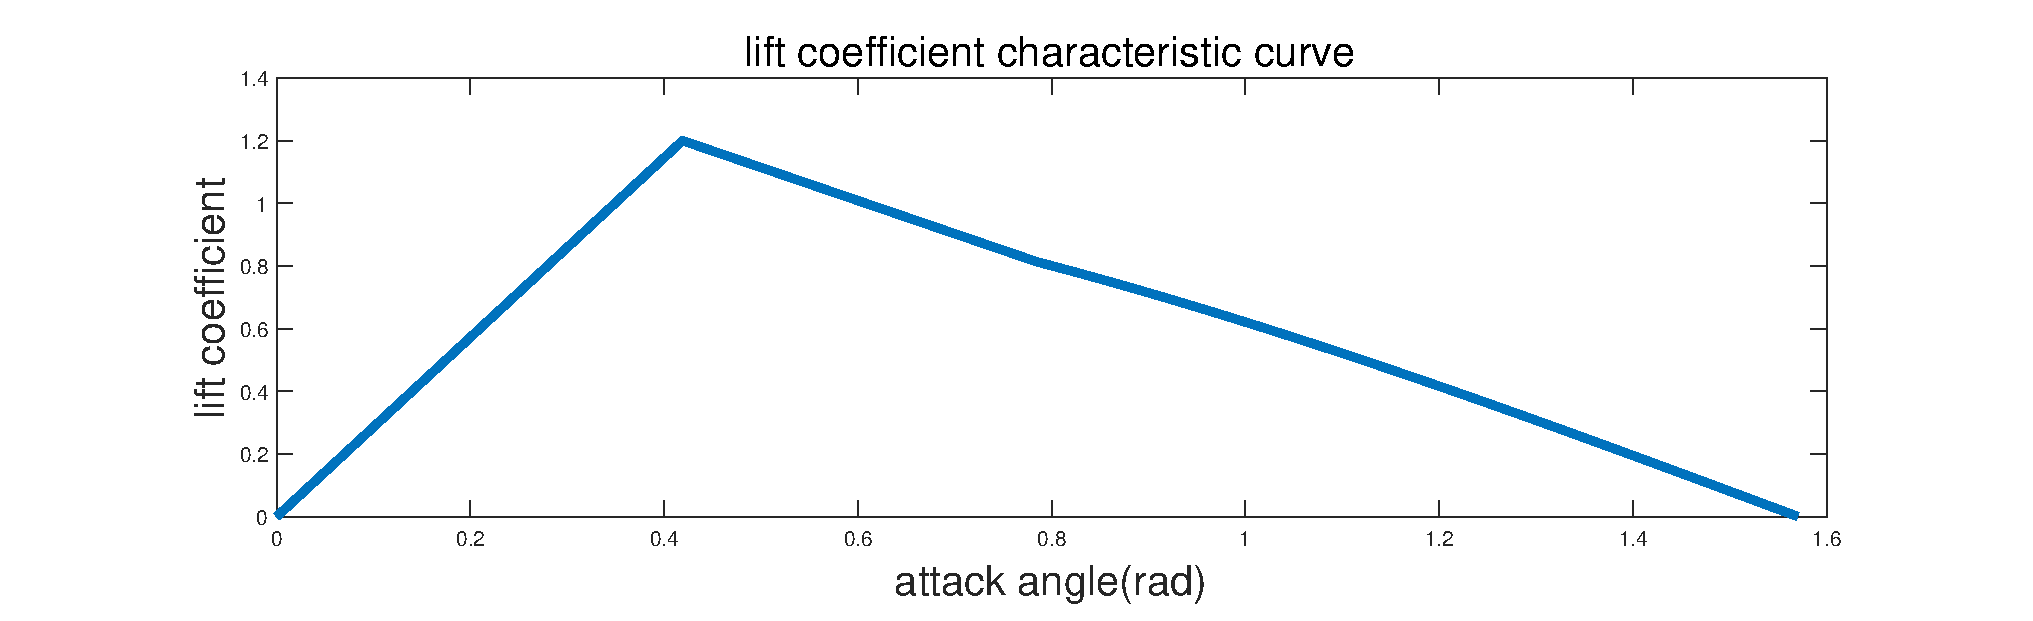
\includegraphics[width=\textwidth]{LiftCoefficient.eps}
\caption{Lift coefficient characteristic curve~\cite{shark}}	
\label{FIG:LiftCoefficient}
\end{figure}
\begin{figure}
\centering
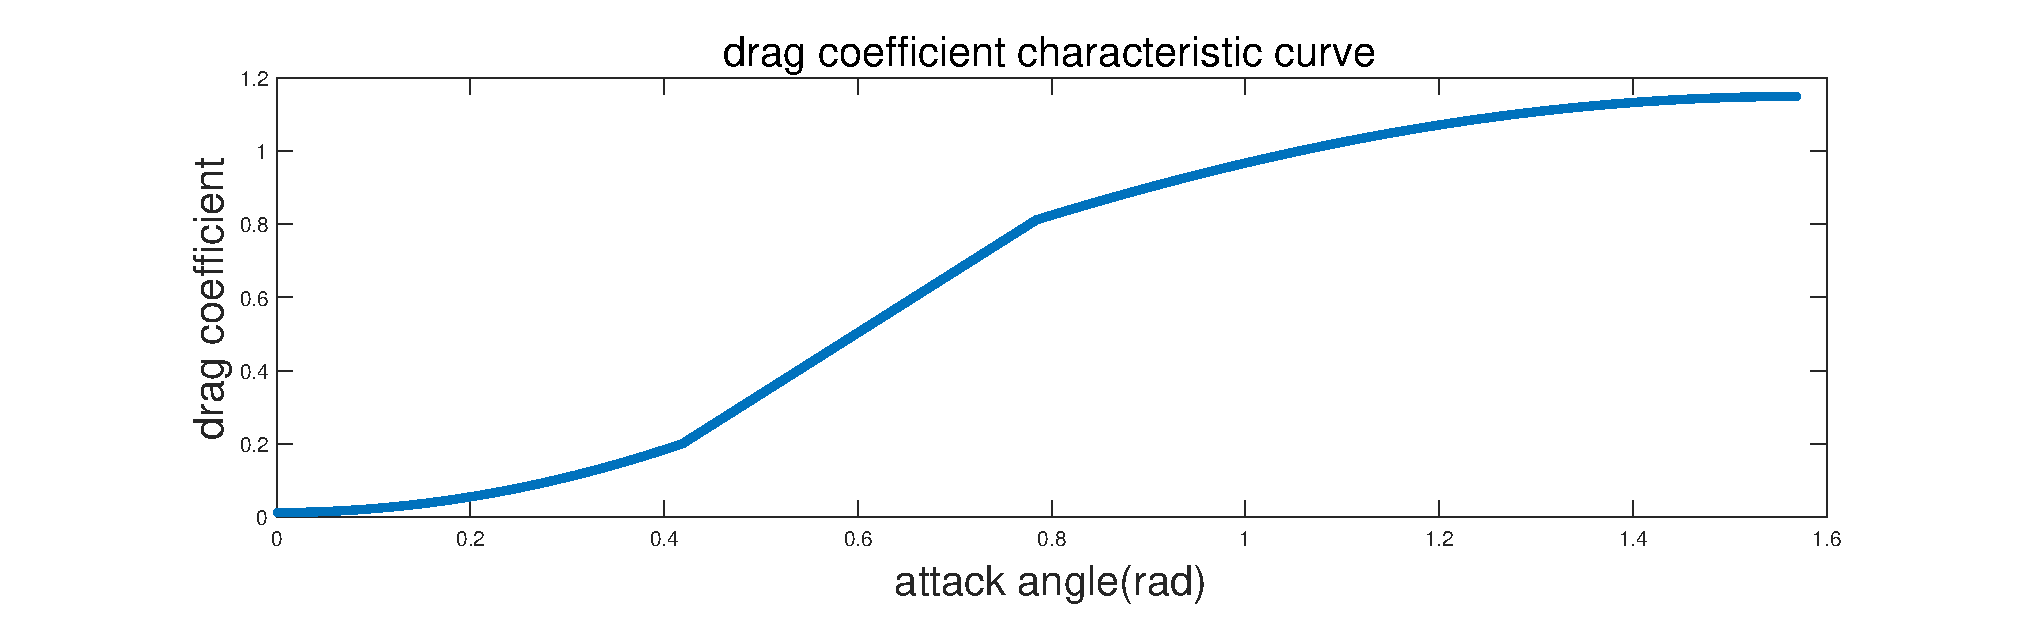
\includegraphics[width=\textwidth]{DragCoefficient.eps}
\caption{Drag coefficient characteristic curve~\cite{shark}}	
\label{FIG:DragCoefficient}
\end{figure}
 
\section{Hydrodynamic Damping on Fins}
The vertical and horizontal fins are installed at the stern of \textit{Snookie} to balance the pitch and yaw instability of forward motion. Regard the vertical fin as two fins on the upper and lower sides and horizontal fin as two fins on the left and right side, that is, four fins are placed symmetrically in difference of $90^{\circ}$. Assume the total hydrodynamic force exerts on the geometric centre of fins. Definitions of fin frames $\left\{ f \right\}$ are illustrated in \ref{FIG:FlowFrameSnookieVerti}, \ref{FIG:FlowFrameSnookieHori}.
\begin{figure}
\centering
\includegraphics[width=\textwidth]{FinFrame.eps}
\caption{Definition of fin frame $\left\{ f \right\}$}	
\label{FIG:FinFrame}
\end{figure}
\begin{figure}
\centering
\includegraphics[width=\textwidth]{FlowFrame1.eps}
\caption{Flow frame $\left\{ flow \right\}$ and hydrodynamic damping for $\alpha\in[0,-\dfrac{\pi}{2}]$}	
\label{FIG:FlowFrame1}
\end{figure}
\begin{figure}
\centering
\includegraphics[width=\textwidth]{FlowFrame2.eps}
\caption{Flow frame $\left\{ flow \right\}$ and hydrodynamic damping for $\alpha\in[-\dfrac{\pi}{2},-\pi]$}	
\label{FIG:FlowFrame2}
\end{figure}
\begin{figure}
\centering
\includegraphics[width=\textwidth]{FlowFrame3.eps}
\caption{Flow frame $\left\{ flow \right\}$ and hydrodynamic damping for $\alpha\in[0,\dfrac{\pi}{2}]$}	
\label{FIG:FlowFrame3}
\end{figure}
\begin{figure}
\centering
\includegraphics[width=\textwidth]{FlowFrame4.eps}
\caption{Flow frame $\left\{ flow \right\}$ and hydrodynamic damping for $\alpha\in[\dfrac{\pi}{2},\pi]$}	
\label{FIG:FlowFrame4}
\end{figure}
\begin{figure}
\centering
\includegraphics[width=\textwidth]{HorizontalFinFrames.eps}
\caption{Fin frames for horizontal fin of \textit{Snoookie}}	
\label{FIG:FlowFrameSnookieVerti}
\end{figure}
\begin{figure}
\centering
\includegraphics[width=0.75\textwidth]{VerticalFinFrames.eps}
\caption{Fin frames for vertical fin of \textit{Snoookie}}	
\label{FIG:FlowFrameSnookieHori}
\end{figure}

The calculation and transformation of hydrodynamic damping of each fin are performed in the following steps: 
\begin{enumerate}
\item The relative generalized velocity vector $\vec{\upsilon}_{r}^{b}$ of our underwater robot is measurable,
where 
\begin{align}
\vec{\upsilon}_{r}^{b}=\begin{pmatrix}
\vec{v}^{b}_{rb/i} \\
\vec{\omega}^{b}_{rb/i}
\end{pmatrix}=
\begin{pmatrix}
u_{r}\\v_{r}\\w_{r}\\p_{r}\\q_{r}\\r_{r}
\end{pmatrix}.
\end{align}
\item Calculate the velocity of the fin center point in body frame $\left\{ b \right\}$ using \ref{EQ:VelocityTransformation}:
\begin{align}
\vec{v}_{r,fin}^{b}=\vec{v}_{r}^{b}+\vec{\omega}_{r}^{b}\times \vec{r}^{b}_{fin},
\end{align}
where $\vec{r}^{b}_{fin}$ is the position vector of a fin geometric center in body frame $\left\{ b \right\}$.
\item Transform the relative velocity $\vec{v}_{r,fin}^{b}$ into the fin frame $\left\{ f \right\}$ using
\begin{align}
\vec{v}_{r,fin}^{f}=\emph{\textbf{R}}_{b}^{f}\vec{v}_{r,fin}^{b}
\end{align}
\item Calculate the attack angle $\alpha$ in the fin frame $\left\{ f \right\}$:
\begin{align}
\alpha=atan2(\vec{v}_{r,fin}^{f}(3),\vec{v}_{r,fin}^{f}(1)).
\end{align}
\item Calculate the rotation matrix $\emph{\textbf{R}}^{flow}_{f}$ from fin frame $\left\{ f \right\}$ to flow frame $\left\{ flow \right\}$ based on the attack angle $\alpha$ according to \ref{EQ:BodyToFlowTrans}.
\item Transform the relative velocity vector of the fin with respect to the fluid $\vec{v}_{r,fin}^{f}$ to flow frame $\left\{ flow \right\}$:
\begin{align}
\vec{v}_{r,fin}^{flow}=\emph{\textbf{R}}^{flow}_{f}\vec{v}_{r,fin}^{f}=\begin{pmatrix}
U_{r,fin}\\0\\0
\end{pmatrix}
\end{align}
\item Determine the lift coefficient $C_{_{L}}$ and drag coefficient $C_{D}$ based on the attack angle $\alpha$ according to the lift coefficient characteristic curve and the drag coefficient curve, respectively.
\item Calculate lift $L_{fin}$ and drag $D_{fin}$ in flow frame $\left\{ flow \right\}$:
\begin{align}
L_{fin}=\dfrac{1}{2}C_{L}S \rho U_{r,fin}^{2},
\end{align}
\begin{align}
D_{fin}=\dfrac{1}{2}C_{D}S \rho U_{r,fin}^{2}.
\end{align}
Define
\begin{align}
\vec{f}^{flow}_{f}=\begin{pmatrix}
D_{fin}\\0\\L_{fin}
\end{pmatrix}.
\end{align}
\item Transfer the lift $L_{fin}$ and drag $D_{fin}$ into body frame $\left\{ b \right\}$ and calculate the resulting moments:
\begin{align}
\vec{f}^{b}_{F}=\emph{\textbf{R}}_{flow}^{f}\emph{\textbf{R}}_{f}^{b}\vec{f}^{flow}_{f}.
\end{align}
The moments of fin in body frame $\left\{ b \right\}$ is calculated as
\begin{align}
\vec{m}^{b}_{F}=\vec{r}_{fin}^{b}\times \vec{f}^{b}_{F}.
\end{align}
\end{enumerate}
\section{Hydrodynamic Damping on Hull}
Calculation of hydrodynamic damping on the hull is much simpler since it shares the same body frame as the underwater robot dynamics. The steps for the calculation of hydrodynamic damping on the hull are as follows:
\begin{enumerate}
\item The relative generalized velocity vector $\vec{\upsilon}_{r}^{b}$ of the underwater robot is measurable,
where 
\begin{align}
\vec{\upsilon}_{r,hull}^{b}=\vec{\upsilon}_{r}^{b}=\begin{pmatrix}
\vec{v}^{b}_{rb/i} \\
\vec{\omega}^{b}_{rb/i}
\end{pmatrix}=
\begin{pmatrix}
u_{r}\\v_{r}\\w_{r}\\p_{r}\\q_{r}\\r_{r}
\end{pmatrix}.
\end{align}
\item Calculate the attack angle $\alpha$ in body frame $\left\{ b \right\}$:
\begin{align}
\alpha=atan2(\vec{v}_{r,hull}^{b}(3),\vec{v}_{r,hull}^{b}(1)).
\end{align}
\item Calculate the rotation matrix $\emph{\textbf{R}}^{flow}_{b}$ from body frame $\left\{ b \right\}$ to flow frame $\left\{ flow \right\}$ based on attack angle $\alpha$ according to \ref{EQ:BodyToFlowTrans}.
\item Transform the relative velocity vector of the hull with respect to the fluid $\vec{v}_{r,hull}^{b}$ to flow frame $\left\{ flow \right\}$:
\begin{align}
\vec{v}_{r,hull}^{flow}=\emph{\textbf{R}}^{flow}_{b}\vec{v}_{r,hull}^{f}=\begin{pmatrix}
U_{r,hull}\\0\\0
\end{pmatrix}
\end{align}
\item Determine the lift coefficient $C_{_{L}}$ and drag coefficient $C_{D}$ based on the attack angle $\alpha$ according to the lift coefficient characteristic curve and the drag coefficient curve, respectively.
\item Calculate lift $L_{hull}$ and drag $D_{hull}$ in flow frame $\left\{ flow \right\}$:
\begin{align}
L_{hull}=\dfrac{1}{2}C_{L}S \rho U_{r,hull}^{2},
\end{align}
\begin{align}
D_{hull}=\dfrac{1}{2}C_{D}S \rho U_{r,hull}^{2}.
\end{align}
Define
\begin{align}
\vec{f}^{flow}_{H}=\begin{pmatrix}
D_{hull}\\0\\L_{hull}
\end{pmatrix}.
\end{align}
\item Transfer the lift $L_{hull}$ and drag $D_{hull}$ into body frame $\left\{ b \right\}$:
\begin{align}
\vec{f}^{b}_{H}=\emph{\textbf{R}}_{flow}^{b}\vec{f}^{flow}_{H}.
\end{align}
Since hull uses the same body-fixed frame with the underwater robot dynamics~(the geometric center of hull), and the exerting point of hydrodynamic damping on hull is the geometric center , lift and drag on hull will not induce any moment.
\end{enumerate}
% \section{Unit Quaternion Representation}
% It is noticeable that singularity problem appears when $\theta=\pm \dfrac{\pi}{2}$ based on Euler angle representation. To avoid this, an alternative four-parameter method on basis of unit quaternions is used. Another advantage in terms of simulation in Matlab/Simulink is that we can limit the range of $\phi$ within $\left[-\pi,\pi \right]$, $\theta$ within $\left[-\dfrac{\pi}{2},\dfrac{\pi}{2}\right]$, and $\psi$ within $\left[-\pi,\pi\right]$. Only four 
% A quaternion $\vec{q}=[\eta,\vec{\varepsilon}^{T}]^{T}$ is a complex number with four elements consisting one real part and three imaginary parts  $\vec{\varepsilon}=[\varepsilon_{1},\varepsilon_{2},\varepsilon_{3}]^{T}$. The set of unit quaternion is defined as 
% \begin{align}
% Q:=\left\lbrace \vec{q}|\vec{q}^{T}\vec{q}=1,\vec{q}=[\eta,\vec{\varepsilon}^{T}]^{T}, \vec{\varepsilon}\in \mathbb{R}^{3}\quad and \quad\eta \in \mathbb{R}\right\rbrace
% \end{align} 
% \begin{align}
% \eta:=cos\left(\dfrac{\beta}{2}\right)
% \end{align}
% \begin{align}
% \vec{\varepsilon}=[\varepsilon_{1},\varepsilon_{2},\varepsilon_{3}]^{T} :=\vec{\lambda}\sin \left(\dfrac{\beta}{2}\right)
% \end{align}
% where $ \vec{\lambda}=[\lambda_{1},\lambda_{2},\lambda_{3}]^{T}$ is a unit vector satisfying 
% \begin{align}
% \vec{\lambda}=\pm \dfrac{\vec{\varepsilon}}{\sqrt{\vec{\varepsilon}^{T}\vec{\varepsilon}}} \quad if \quad {\sqrt{\vec{\varepsilon}^{T}\vec{\varepsilon}}} \neq 0
% \end{align}
% 
% The unit quaternion can be expressed in the following form
% \begin{align}
% \vec{q}=\begin{pmatrix}
% \eta\\ \varepsilon_{1} \\ \varepsilon_{2} \\ \varepsilon_{3}
% \end{pmatrix}
% \end{align}
% \begin{align}
% \eta^{2}+\varepsilon_{1}^{2}+\varepsilon_{2}^{2}+
% \varepsilon_{3}^{2}=1
% \end{align}
% Based on the new representation method, the angular velocity transformation matrix and linear velocity transformation matrix can be reparametrized with unit quaternion.  
% \begin{align}
% \dot{\vec{p}}_{b/i}^{i}=\emph{\textbf{R}}_{b}^{i}(\vec{q})\vec{\upsilon}_{b/i}^{b}
% \end{align}
% \begin{align}
% \dot{\vec{q}}=\emph{\textbf{T}}_{q}(\vec{q})\vec{\omega}_{b/i}^{b}
% \end{align}
% The 6DOF Kinematic equation can be written as follows:
% \begin{align}
% \dot{\vec{\eta}}=\emph{\textbf{J}}_{q}(\vec{\eta})\vec{\upsilon} \Leftrightarrow
% \begin{pmatrix}
% \dot{\vec{p}}_{b/i}^{i} \\ \dot{\vec{q}}
% \end{pmatrix}
% =
% \begin{pmatrix}
% \emph{\textbf{R}}_{b}^{i}(\vec{q})&\vec{0}_{3\times3} \\
% \vec{0}_{4\times3}& \emph{\textbf{T}}_{q}(\vec{q})
% \end{pmatrix}
% \begin{pmatrix}
% \vec{\upsilon}_{b/i}^{b} \\
% \vec{\omega}_{b/i}^{b} 
% \end{pmatrix}
% \end{align}
% where $ \vec{\eta}=[x,y,z,\eta,\varepsilon_{1},\varepsilon_{2},\varepsilon_{3}]^{T} \in \mathbb{R}^{7}$, $\vec{\upsilon} \in \mathbb{R}^{6}$ and $\emph{\textbf{J}}_{q} \in \mathbb{R}^{7\times 6}$.
% \subsection{Implementation Problem}
% Suppose a differential equation: 
% \begin{align}
% y^{'}=f\left(t,y(t)\right) 
% \end{align}
% where $y(t_{0})=y_{0}$
% \begin{align}
% y_{n+1}=y_{n}+hf(t_{n},y_{n})
% \end{align}
% where $h$ is the step size 
% in our case 
% \begin{align}
% \dot{\vec{q}}=\emph{\textbf{T}}_{q}(\vec{q})\vec{\omega}^{b}_{b/i}
% \end{align}
% \begin{align}
% \vec{q}_{n+1}=\vec{q}_{n}+h\emph{\textbf{T}}_{q}(\vec{q}_{n})\vec{\omega}^{b}_{b/i,n}
% \end{align}
% section{Interpolation of Feedback Gain}
% With LQR Scheduling method, we linearize the underwater robot  dynamics according to some scheduling variables. We choose some schedule variable 
% 
% The matrix is defined as a function of three independent scheduling variables:
% \begin{align}
% x=\left[x_{1},x_{2},x_{3},\ldots{},x_{i},x_{i+1},\ldots{},x_{n}\right]
% \end{align}
% \begin{align}
% y=\left[y_{1},y_{2},y_{3},\ldots{},y_{j},y_{j+1},\ldots{},y_{m}\right]
% \end{align}
% \begin{align}
% z=\left[z_{1},z_{2},z_{3},\ldots{},z_{k},z_{k+1},\ldots{},y_{p}\right]
% \end{align}
% For given values of $x$,$y$ and $z$, eight matrices are interpolated. Then for $x_{i}<x<x_{i+1}$, $y_{j}<y<$, $z_{k}<z<z_{k+1}$.
% 
% We interpolate in such a way that 
% \begin{align}
% \left(1-\lambda_{z}\right)\lbrace (1-\lambda_{y})[(1-\lambda_{x})M(x_{i},y_{j},z_{k})+\lambda_{x}M(x_{i+1},y_{j},z_{k}) \nonumber \\
% +\lambda_{y}[(1-\lambda_{x})M(x_{i},y_{j+1},z_{k})+\lambda_{x}M(x_{i+1},y_{j+1},z_{k})
% ]\rbrace \nonumber \\
% +\lambda_{z}\lbrace (1-\lambda_{y})[(1-\lambda_{x})M(x_{i},y_{j},z_{k+1})+\lambda_{x}M(x_{i+1},y_{j},z_{k+1})
% \nonumber \\
% +\lambda_{y}[(1-\lambda_{x})M(x_{i},y_{j+1},z_{k+1})+\lambda_{x}M(x_{i+1},y_{j+1},z_{k+1})
% ]\rbrace 
% \end{align}
% Multilevel convex combination 
% where the interpolation fractions are denoted by
% \begin{align}
% \lambda_{x}=(x-x_{i})/(x_{i+1}-x_{i})
% \end{align}
% \begin{align}
% \lambda_{y}=(y-y_{j})/(y_{j+1}-y_{j})
% \end{align}
% \begin{align}
% \lambda_{z}=(z-z_{k})/(z_{k+1}-z_{k})
% \end{align}
